% Options for packages loaded elsewhere
% Options for packages loaded elsewhere
\PassOptionsToPackage{unicode}{hyperref}
\PassOptionsToPackage{hyphens}{url}
\PassOptionsToPackage{dvipsnames,svgnames,x11names}{xcolor}
%
\documentclass[
  letterpaper,
  DIV=11,
  numbers=noendperiod]{scrartcl}
\usepackage{xcolor}
\usepackage{amsmath,amssymb}
\setcounter{secnumdepth}{-\maxdimen} % remove section numbering
\usepackage{iftex}
\ifPDFTeX
  \usepackage[T1]{fontenc}
  \usepackage[utf8]{inputenc}
  \usepackage{textcomp} % provide euro and other symbols
\else % if luatex or xetex
  \usepackage{unicode-math} % this also loads fontspec
  \defaultfontfeatures{Scale=MatchLowercase}
  \defaultfontfeatures[\rmfamily]{Ligatures=TeX,Scale=1}
\fi
\usepackage{lmodern}
\ifPDFTeX\else
  % xetex/luatex font selection
\fi
% Use upquote if available, for straight quotes in verbatim environments
\IfFileExists{upquote.sty}{\usepackage{upquote}}{}
\IfFileExists{microtype.sty}{% use microtype if available
  \usepackage[]{microtype}
  \UseMicrotypeSet[protrusion]{basicmath} % disable protrusion for tt fonts
}{}
\makeatletter
\@ifundefined{KOMAClassName}{% if non-KOMA class
  \IfFileExists{parskip.sty}{%
    \usepackage{parskip}
  }{% else
    \setlength{\parindent}{0pt}
    \setlength{\parskip}{6pt plus 2pt minus 1pt}}
}{% if KOMA class
  \KOMAoptions{parskip=half}}
\makeatother
% Make \paragraph and \subparagraph free-standing
\makeatletter
\ifx\paragraph\undefined\else
  \let\oldparagraph\paragraph
  \renewcommand{\paragraph}{
    \@ifstar
      \xxxParagraphStar
      \xxxParagraphNoStar
  }
  \newcommand{\xxxParagraphStar}[1]{\oldparagraph*{#1}\mbox{}}
  \newcommand{\xxxParagraphNoStar}[1]{\oldparagraph{#1}\mbox{}}
\fi
\ifx\subparagraph\undefined\else
  \let\oldsubparagraph\subparagraph
  \renewcommand{\subparagraph}{
    \@ifstar
      \xxxSubParagraphStar
      \xxxSubParagraphNoStar
  }
  \newcommand{\xxxSubParagraphStar}[1]{\oldsubparagraph*{#1}\mbox{}}
  \newcommand{\xxxSubParagraphNoStar}[1]{\oldsubparagraph{#1}\mbox{}}
\fi
\makeatother


\usepackage{longtable,booktabs,array}
\usepackage{calc} % for calculating minipage widths
% Correct order of tables after \paragraph or \subparagraph
\usepackage{etoolbox}
\makeatletter
\patchcmd\longtable{\par}{\if@noskipsec\mbox{}\fi\par}{}{}
\makeatother
% Allow footnotes in longtable head/foot
\IfFileExists{footnotehyper.sty}{\usepackage{footnotehyper}}{\usepackage{footnote}}
\makesavenoteenv{longtable}
\usepackage{graphicx}
\makeatletter
\newsavebox\pandoc@box
\newcommand*\pandocbounded[1]{% scales image to fit in text height/width
  \sbox\pandoc@box{#1}%
  \Gscale@div\@tempa{\textheight}{\dimexpr\ht\pandoc@box+\dp\pandoc@box\relax}%
  \Gscale@div\@tempb{\linewidth}{\wd\pandoc@box}%
  \ifdim\@tempb\p@<\@tempa\p@\let\@tempa\@tempb\fi% select the smaller of both
  \ifdim\@tempa\p@<\p@\scalebox{\@tempa}{\usebox\pandoc@box}%
  \else\usebox{\pandoc@box}%
  \fi%
}
% Set default figure placement to htbp
\def\fps@figure{htbp}
\makeatother


% definitions for citeproc citations
\NewDocumentCommand\citeproctext{}{}
\NewDocumentCommand\citeproc{mm}{%
  \begingroup\def\citeproctext{#2}\cite{#1}\endgroup}
\makeatletter
 % allow citations to break across lines
 \let\@cite@ofmt\@firstofone
 % avoid brackets around text for \cite:
 \def\@biblabel#1{}
 \def\@cite#1#2{{#1\if@tempswa , #2\fi}}
\makeatother
\newlength{\cslhangindent}
\setlength{\cslhangindent}{1.5em}
\newlength{\csllabelwidth}
\setlength{\csllabelwidth}{3em}
\newenvironment{CSLReferences}[2] % #1 hanging-indent, #2 entry-spacing
 {\begin{list}{}{%
  \setlength{\itemindent}{0pt}
  \setlength{\leftmargin}{0pt}
  \setlength{\parsep}{0pt}
  % turn on hanging indent if param 1 is 1
  \ifodd #1
   \setlength{\leftmargin}{\cslhangindent}
   \setlength{\itemindent}{-1\cslhangindent}
  \fi
  % set entry spacing
  \setlength{\itemsep}{#2\baselineskip}}}
 {\end{list}}
\usepackage{calc}
\newcommand{\CSLBlock}[1]{\hfill\break\parbox[t]{\linewidth}{\strut\ignorespaces#1\strut}}
\newcommand{\CSLLeftMargin}[1]{\parbox[t]{\csllabelwidth}{\strut#1\strut}}
\newcommand{\CSLRightInline}[1]{\parbox[t]{\linewidth - \csllabelwidth}{\strut#1\strut}}
\newcommand{\CSLIndent}[1]{\hspace{\cslhangindent}#1}



\setlength{\emergencystretch}{3em} % prevent overfull lines

\providecommand{\tightlist}{%
  \setlength{\itemsep}{0pt}\setlength{\parskip}{0pt}}



 


\usepackage{amsfonts}
\usepackage{amsmath}
\usepackage{braket}
\KOMAoption{captions}{tableheading}
\makeatletter
\@ifpackageloaded{caption}{}{\usepackage{caption}}
\AtBeginDocument{%
\ifdefined\contentsname
  \renewcommand*\contentsname{Table of contents}
\else
  \newcommand\contentsname{Table of contents}
\fi
\ifdefined\listfigurename
  \renewcommand*\listfigurename{List of Figures}
\else
  \newcommand\listfigurename{List of Figures}
\fi
\ifdefined\listtablename
  \renewcommand*\listtablename{List of Tables}
\else
  \newcommand\listtablename{List of Tables}
\fi
\ifdefined\figurename
  \renewcommand*\figurename{Figure}
\else
  \newcommand\figurename{Figure}
\fi
\ifdefined\tablename
  \renewcommand*\tablename{Table}
\else
  \newcommand\tablename{Table}
\fi
}
\@ifpackageloaded{float}{}{\usepackage{float}}
\floatstyle{ruled}
\@ifundefined{c@chapter}{\newfloat{codelisting}{h}{lop}}{\newfloat{codelisting}{h}{lop}[chapter]}
\floatname{codelisting}{Listing}
\newcommand*\listoflistings{\listof{codelisting}{List of Listings}}
\makeatother
\makeatletter
\makeatother
\makeatletter
\@ifpackageloaded{caption}{}{\usepackage{caption}}
\@ifpackageloaded{subcaption}{}{\usepackage{subcaption}}
\makeatother
\usepackage{bookmark}
\IfFileExists{xurl.sty}{\usepackage{xurl}}{} % add URL line breaks if available
\urlstyle{same}
\hypersetup{
  colorlinks=true,
  linkcolor={blue},
  filecolor={Maroon},
  citecolor={Blue},
  urlcolor={Blue},
  pdfcreator={LaTeX via pandoc}}


\author{}
\date{}
\begin{document}


\subsection{02/11/2026}\label{section}

Had presentation, think it went decently. \#\#\# Quick after
presentation scratch notes:

Presentation felt decent, Went a bit quicker speech wise than i wanted
to Throat scratchy didnt help Was under time Questions: - multiple
recurrence, yes, inc side note on small system reccurence - how quantum
error correction, gave practiced answer - logical qubit size, gave
default answer for simple answer, wasnt real logical qbit answer, but i
made clear i was talking about minimum example - real examples of this
model, i gave impurity in condesned matter crystal, he one upped w/water
molecules

Last 3 were prof, hes a quantum computational guy

Prof was guy who wants to show hes smarter than you, i think i held my
own, the power of ``this is beyond the scope but\ldots{}''

I think my minor jokes (i.e big ugly correlation matrix) helped, i saw
minor smiles at that

Looking at audience, did better than most i think, but still looked at
slides a bit too much

Didnt pause for breath enough i think so went a bit fast

\subsection{04/11/2026}\label{section-1}

\subsubsection{supervisor meeting}\label{supervisor-meeting}

Quickly recapped presentation - went fine, didn't need to cover that too
much. Reiterated next steps of implementing metrics, then can examine
memory effects. Discussed potential things that can be examined w/memory
effects, discussion was a touch rambly/wide ranging but provided useful
intuition inc:

\begin{itemize}
\tightlist
\item
  adding narrow peak to spectral function - structure adds memory
  effects
\item
  relationship between fourrier transform of spectral function and
  memory effects (system/bath correlations?
  \$\mathcal{F}(J(\omega))\cdot f \approx \$ correlations)
\item
  need to seperate effects of structure and overall coupling - need to
  normalize coupling strength of spectral function
\item
  discussed some of David's work w/mpemba effect - discussed reentrance
  time and the gap between initially thermalized state and maximum
  deviation from that - this may be a useful ``mini-memory metric''
\item
  Note - to extract thermalization numerically, can diagonalize
  \(\Lambda \rho_{therm} = \rho_{therm}\), when \(\rho_{therm}\)
  stabilises, is thermalized
\item
  can map out maximum deviation metric over \(\mu\) for \(\beta=10\)
  (see (Strachan, Purkayastha, and Clark 2025) fig 2) - fig 2 phase
  diagram may be interesting to map out metrics over in general? tbd
\end{itemize}

immediate plan:

\begin{itemize}
\tightlist
\item
  implement numeric thermalization determination from map
\item
  implement deviation gap mini metric
\item
  implement memory kernel def
\item
  examine metrics over \(\mu\) as outlined above
\end{itemize}

\subsection{07/11/2026}\label{section-2}

Finally returning to actual work on this project.

\subsubsection{Code work: eigenvector thermalization
computation}\label{code-work-eigenvector-thermalization-computation}

Going to first try to implement the eigen method for thermalization
determination. Unsure exactly how this will work; there are dynamic map
matrices for every time step, and given these are \(2\times 2\)
matrices, i'd assume they have 2 eigenvectors. Going to quickly examine
what these look like and see if there's any obvious stabilisation. This
spits out 2 eigenvectors for each timestep of the dynamic map. Comparing
\(|\vec{v(t_{n})}-\vec{v(t_{n-1})}|\) for the first and second
eigenvectors respectively yields:

\begin{figure}

\centering{

\pandocbounded{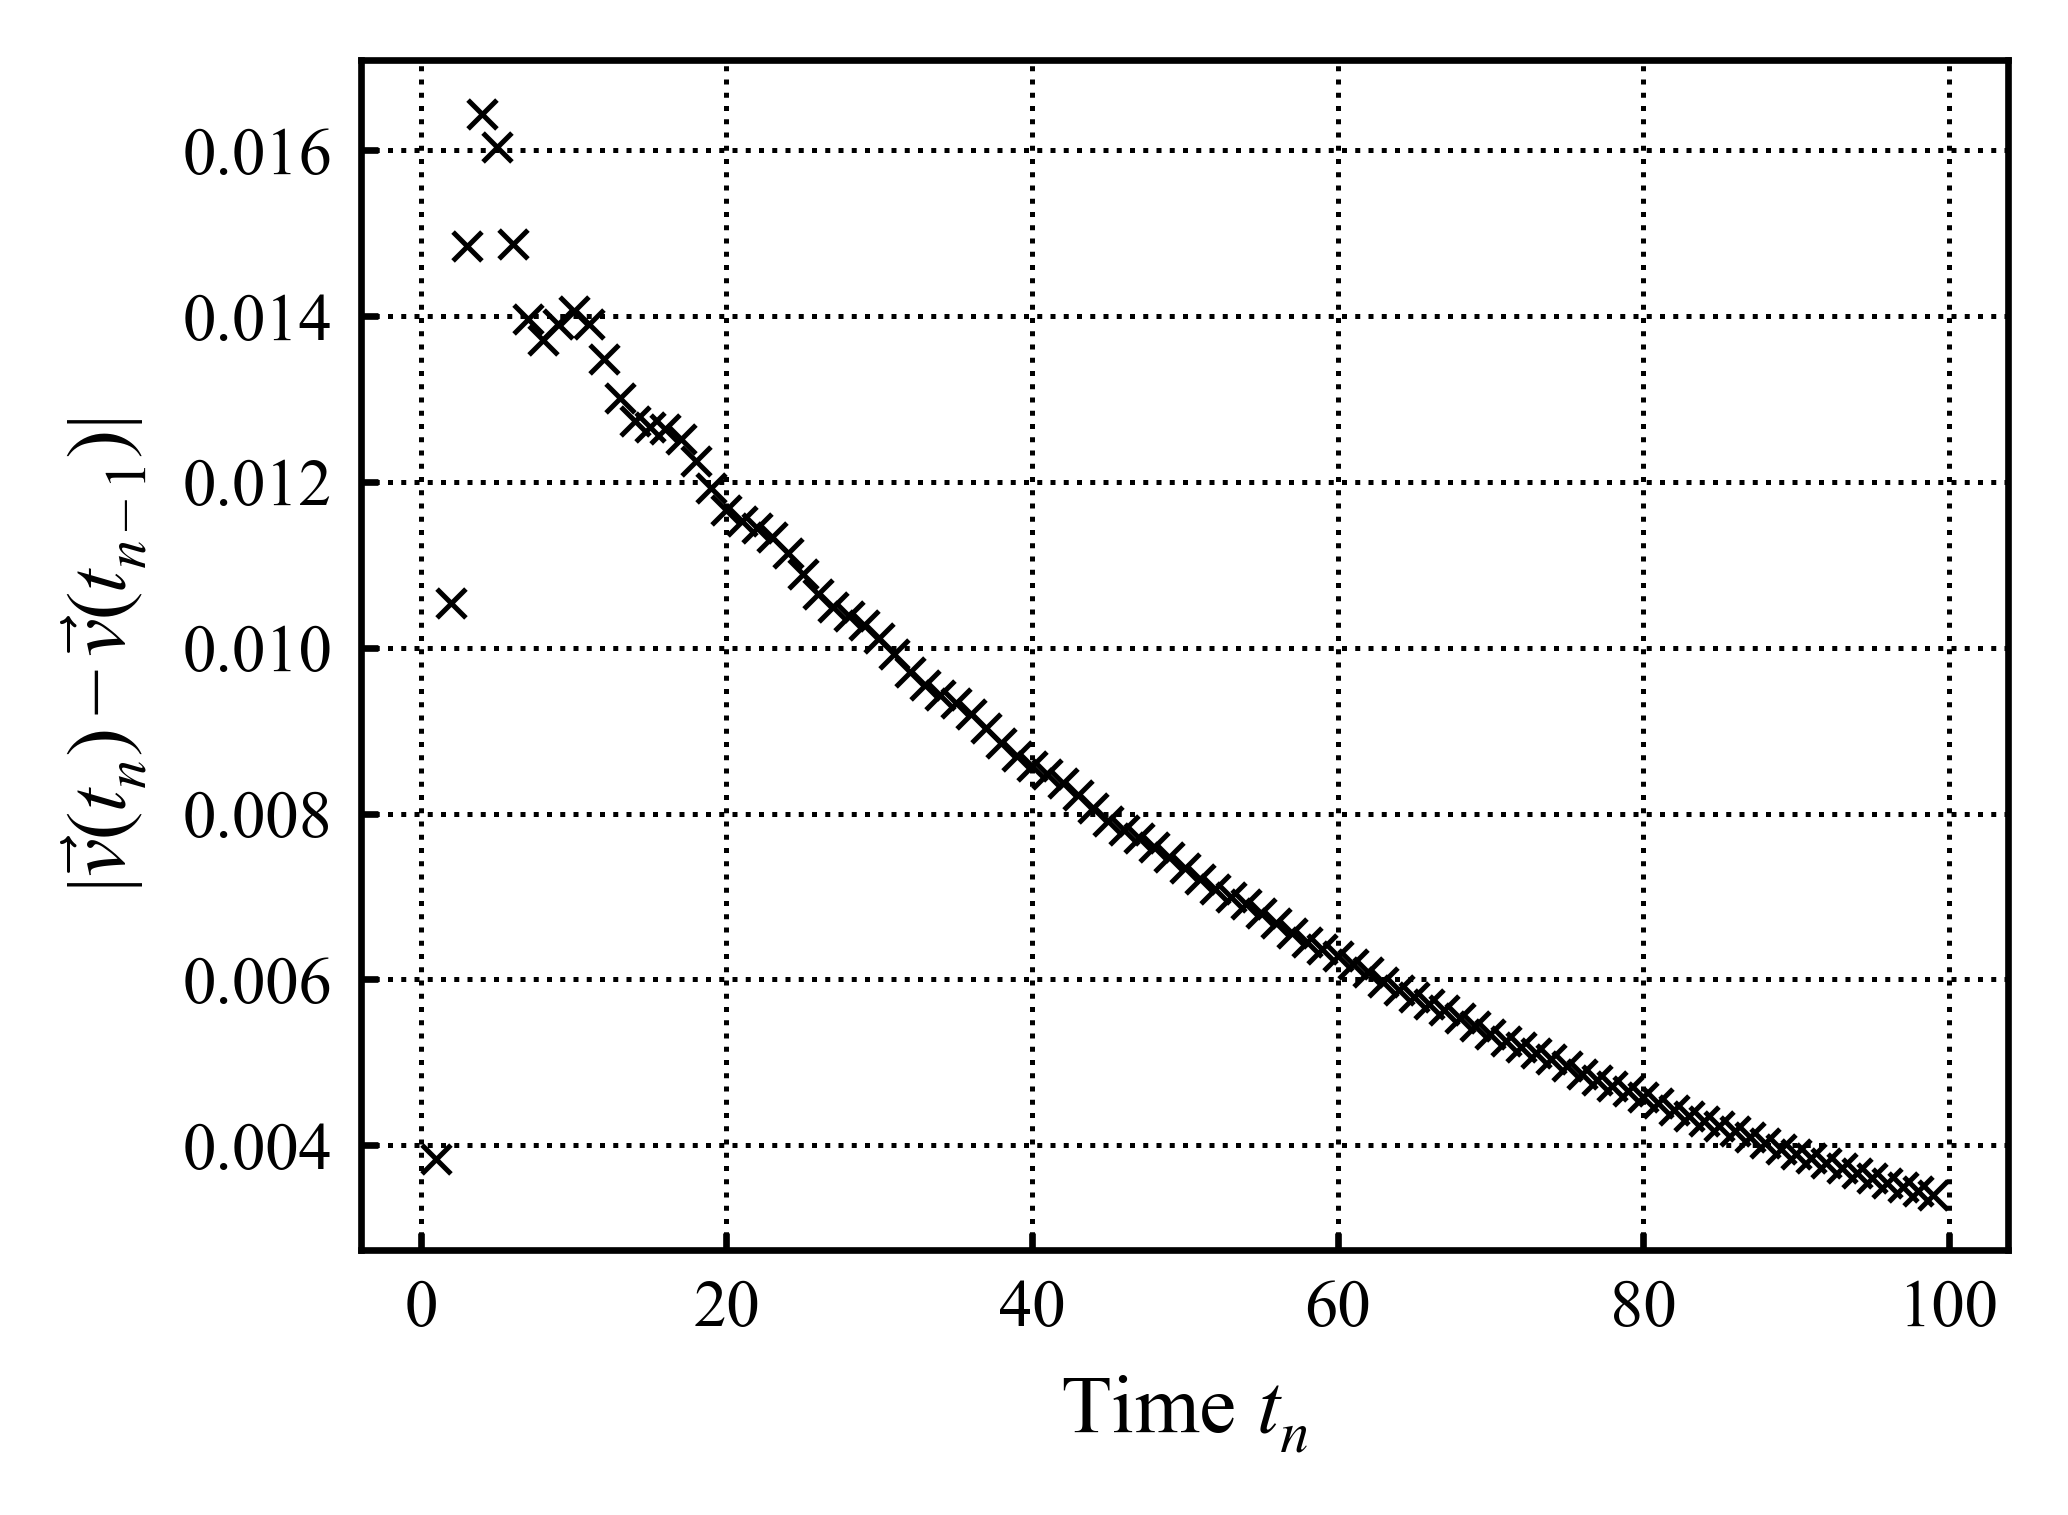
\includegraphics[keepaspectratio]{figures/eigenconvergence1.png}}

}

\caption{\label{fig-eigenconvergence1}First eigenvector convergence}

\end{figure}%

\begin{figure}

\centering{

\pandocbounded{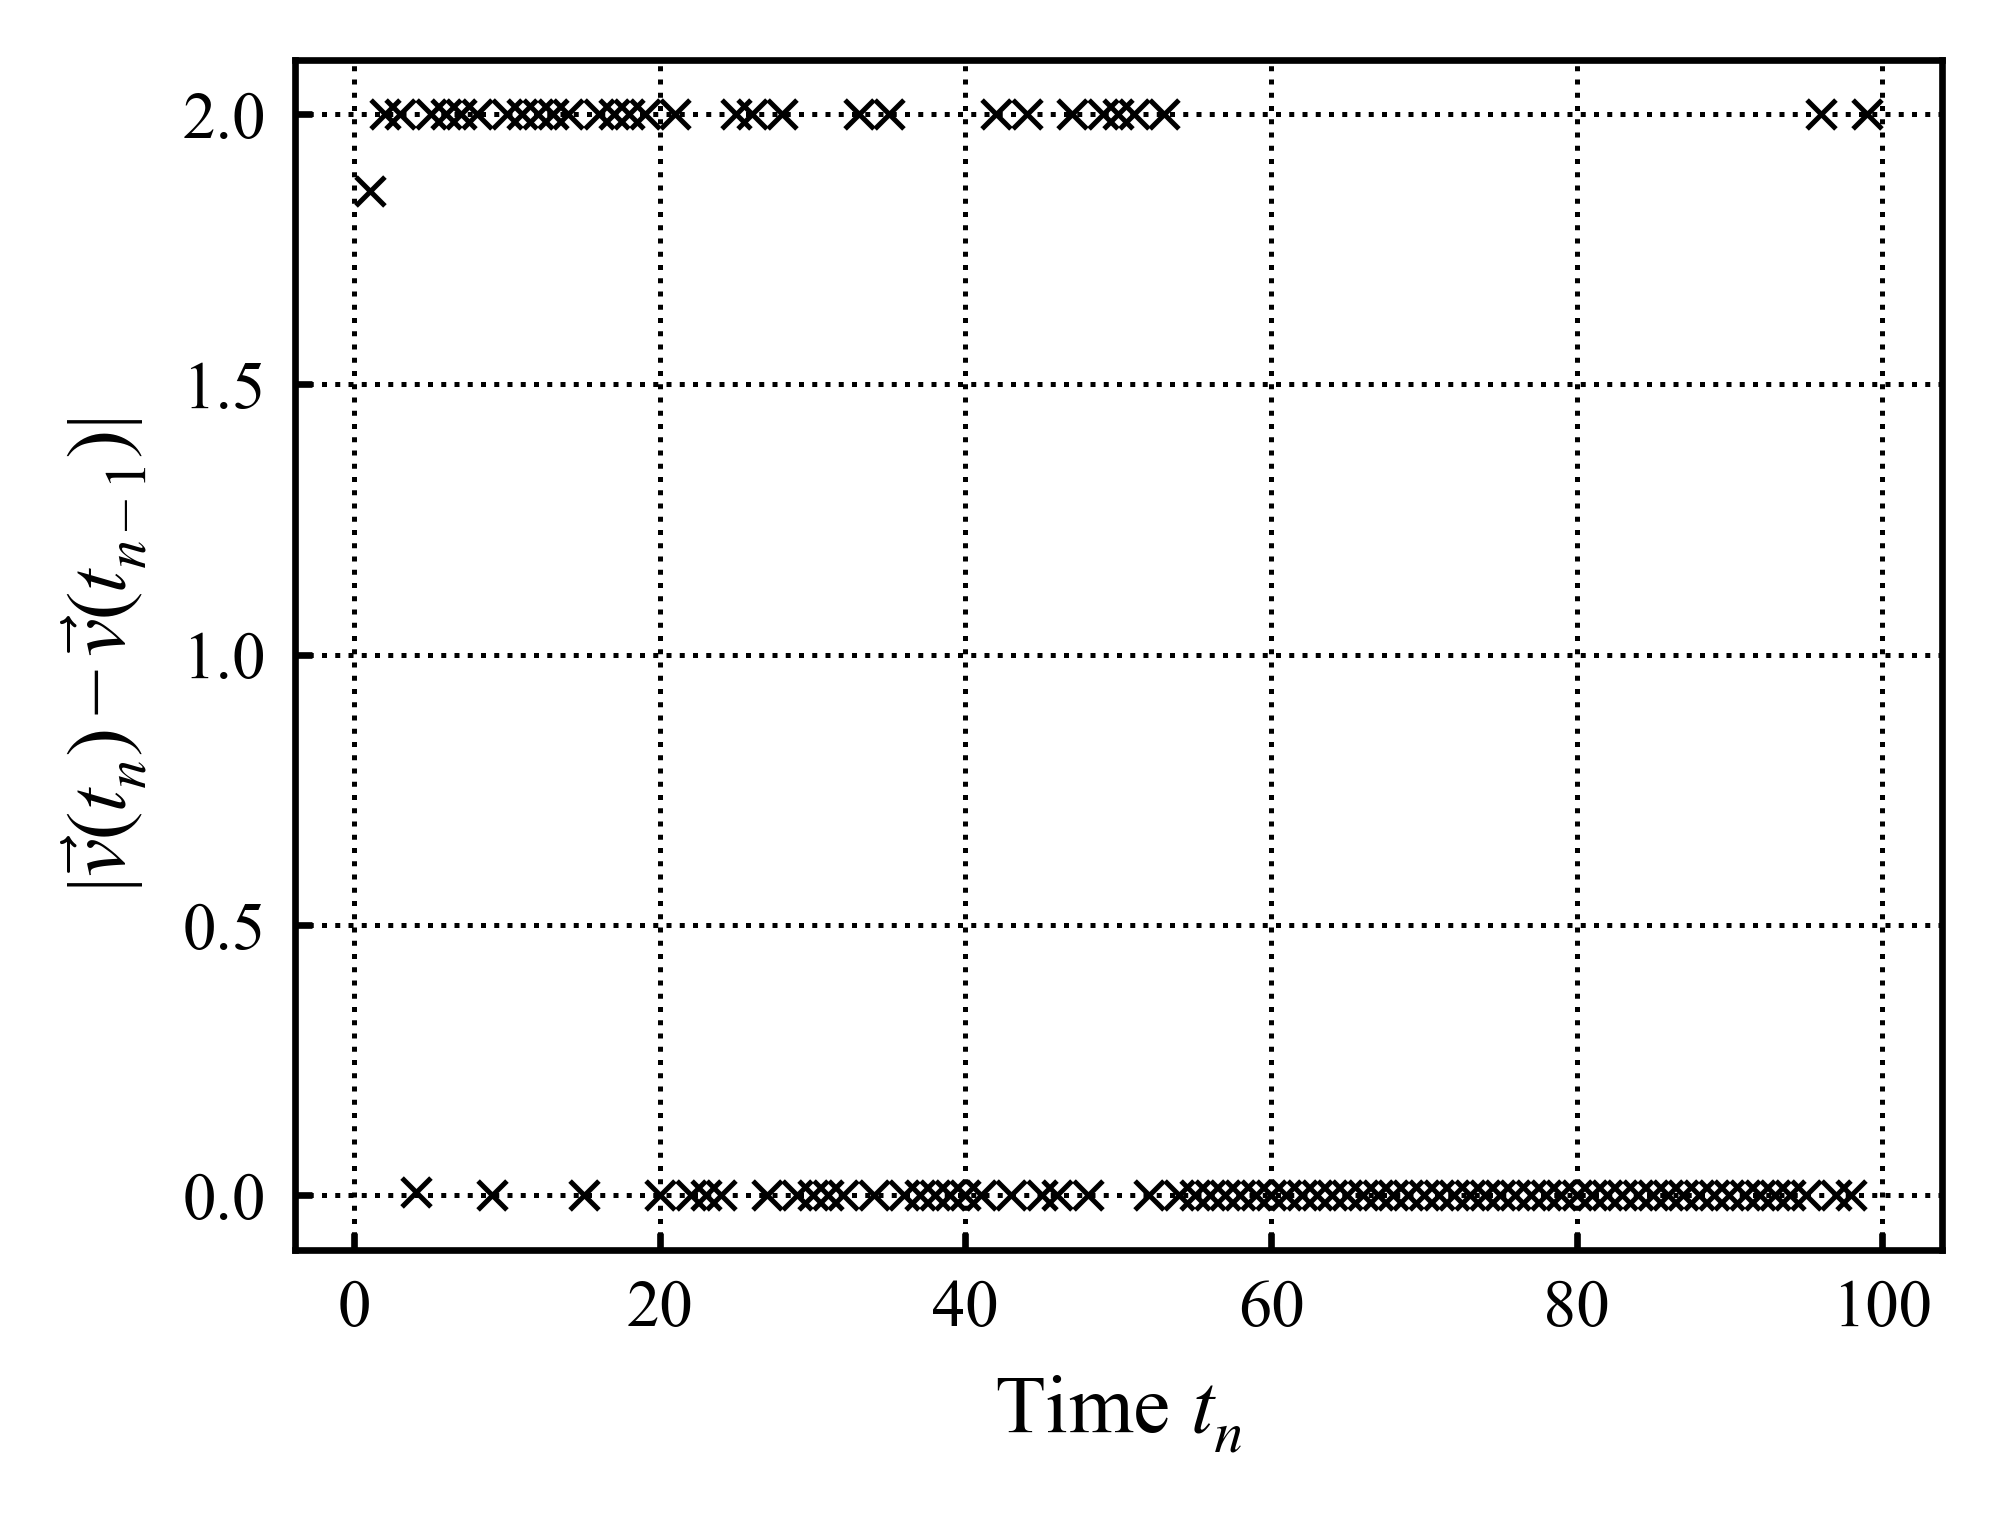
\includegraphics[keepaspectratio]{figures/eigenconvergence2.png}}

}

\caption{\label{fig-eigenconvergence2}Second eigenvector convergence}

\end{figure}%

hmm, first eigenvector generally converges, second doesn't. The fact
Figure~\ref{fig-eigenconvergence2} seems to flip between
\(|\vec{v(t_{n})}-\vec{v(t_{n-1})}|\approx 0, 2\) is suspicious. I could
just use the first eigenvector, but I want to make sure this isn't some
artefact or smth that could come back to haunt me. The eigenvectors
numpy is spitting out aren't normalized, so will start with that; the
Figure~\ref{fig-eigenconvergence2} flipping may simply be the
eigenvector pointing in different directions. Normalization doesn't help
too much:

\begin{figure}

\centering{

\pandocbounded{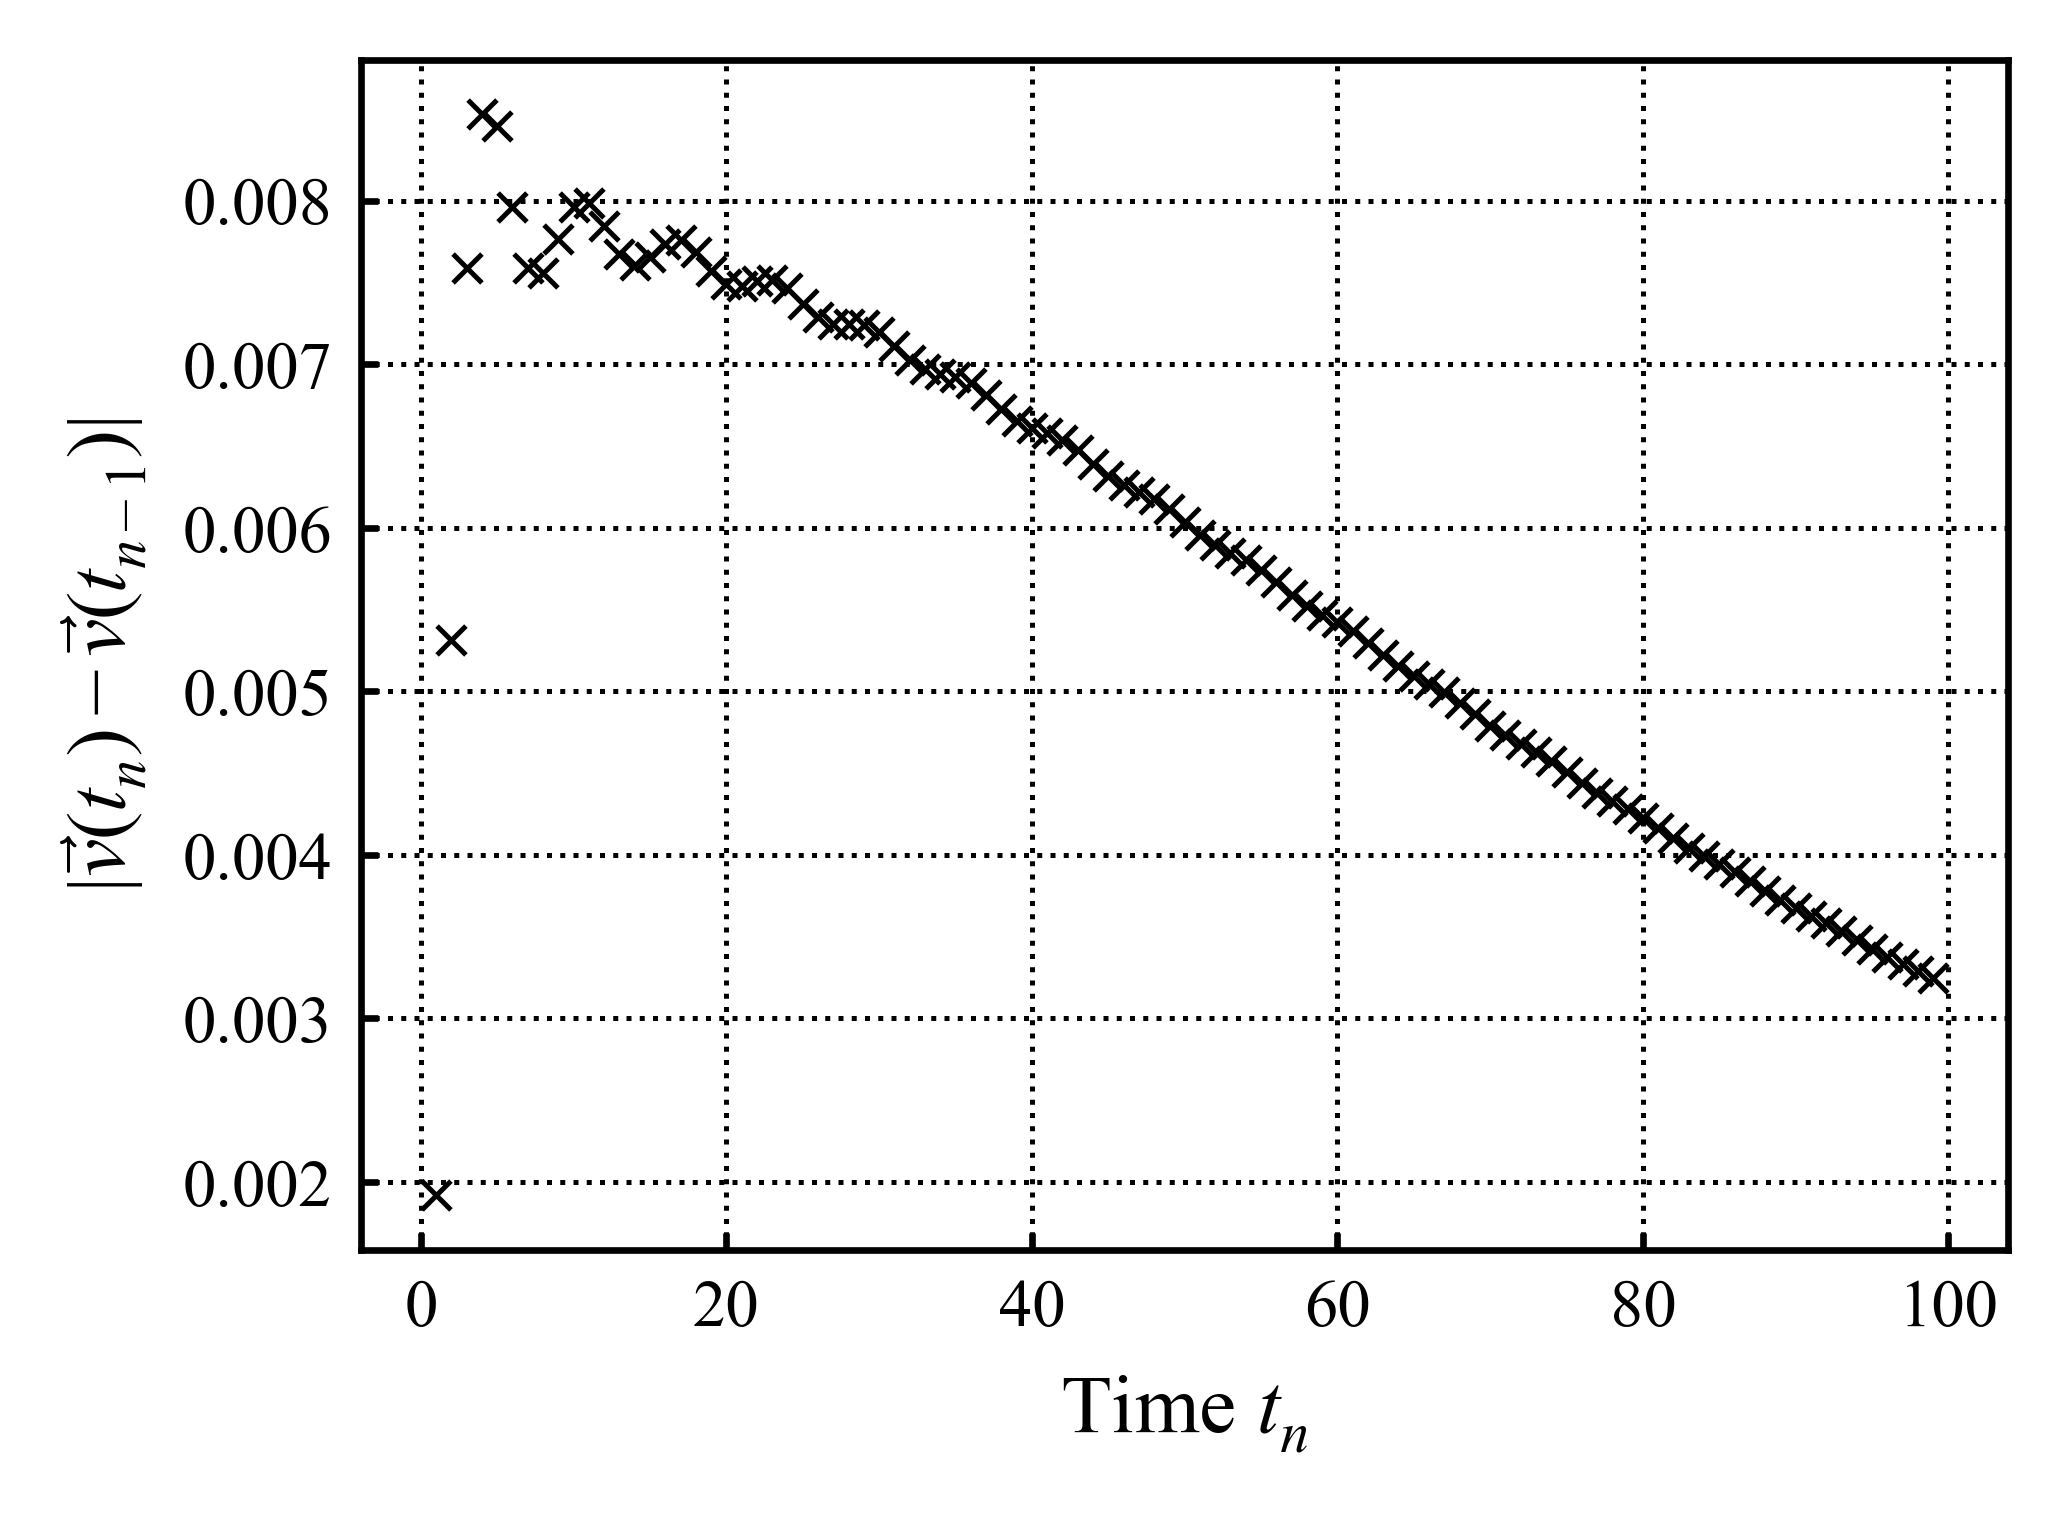
\includegraphics[keepaspectratio]{figures/eigenconvergence1Normed.png}}

}

\caption{\label{fig-eigenconvergence1Normed}Normalized first eigenvector
convergence}

\end{figure}%

\begin{figure}

\centering{

\pandocbounded{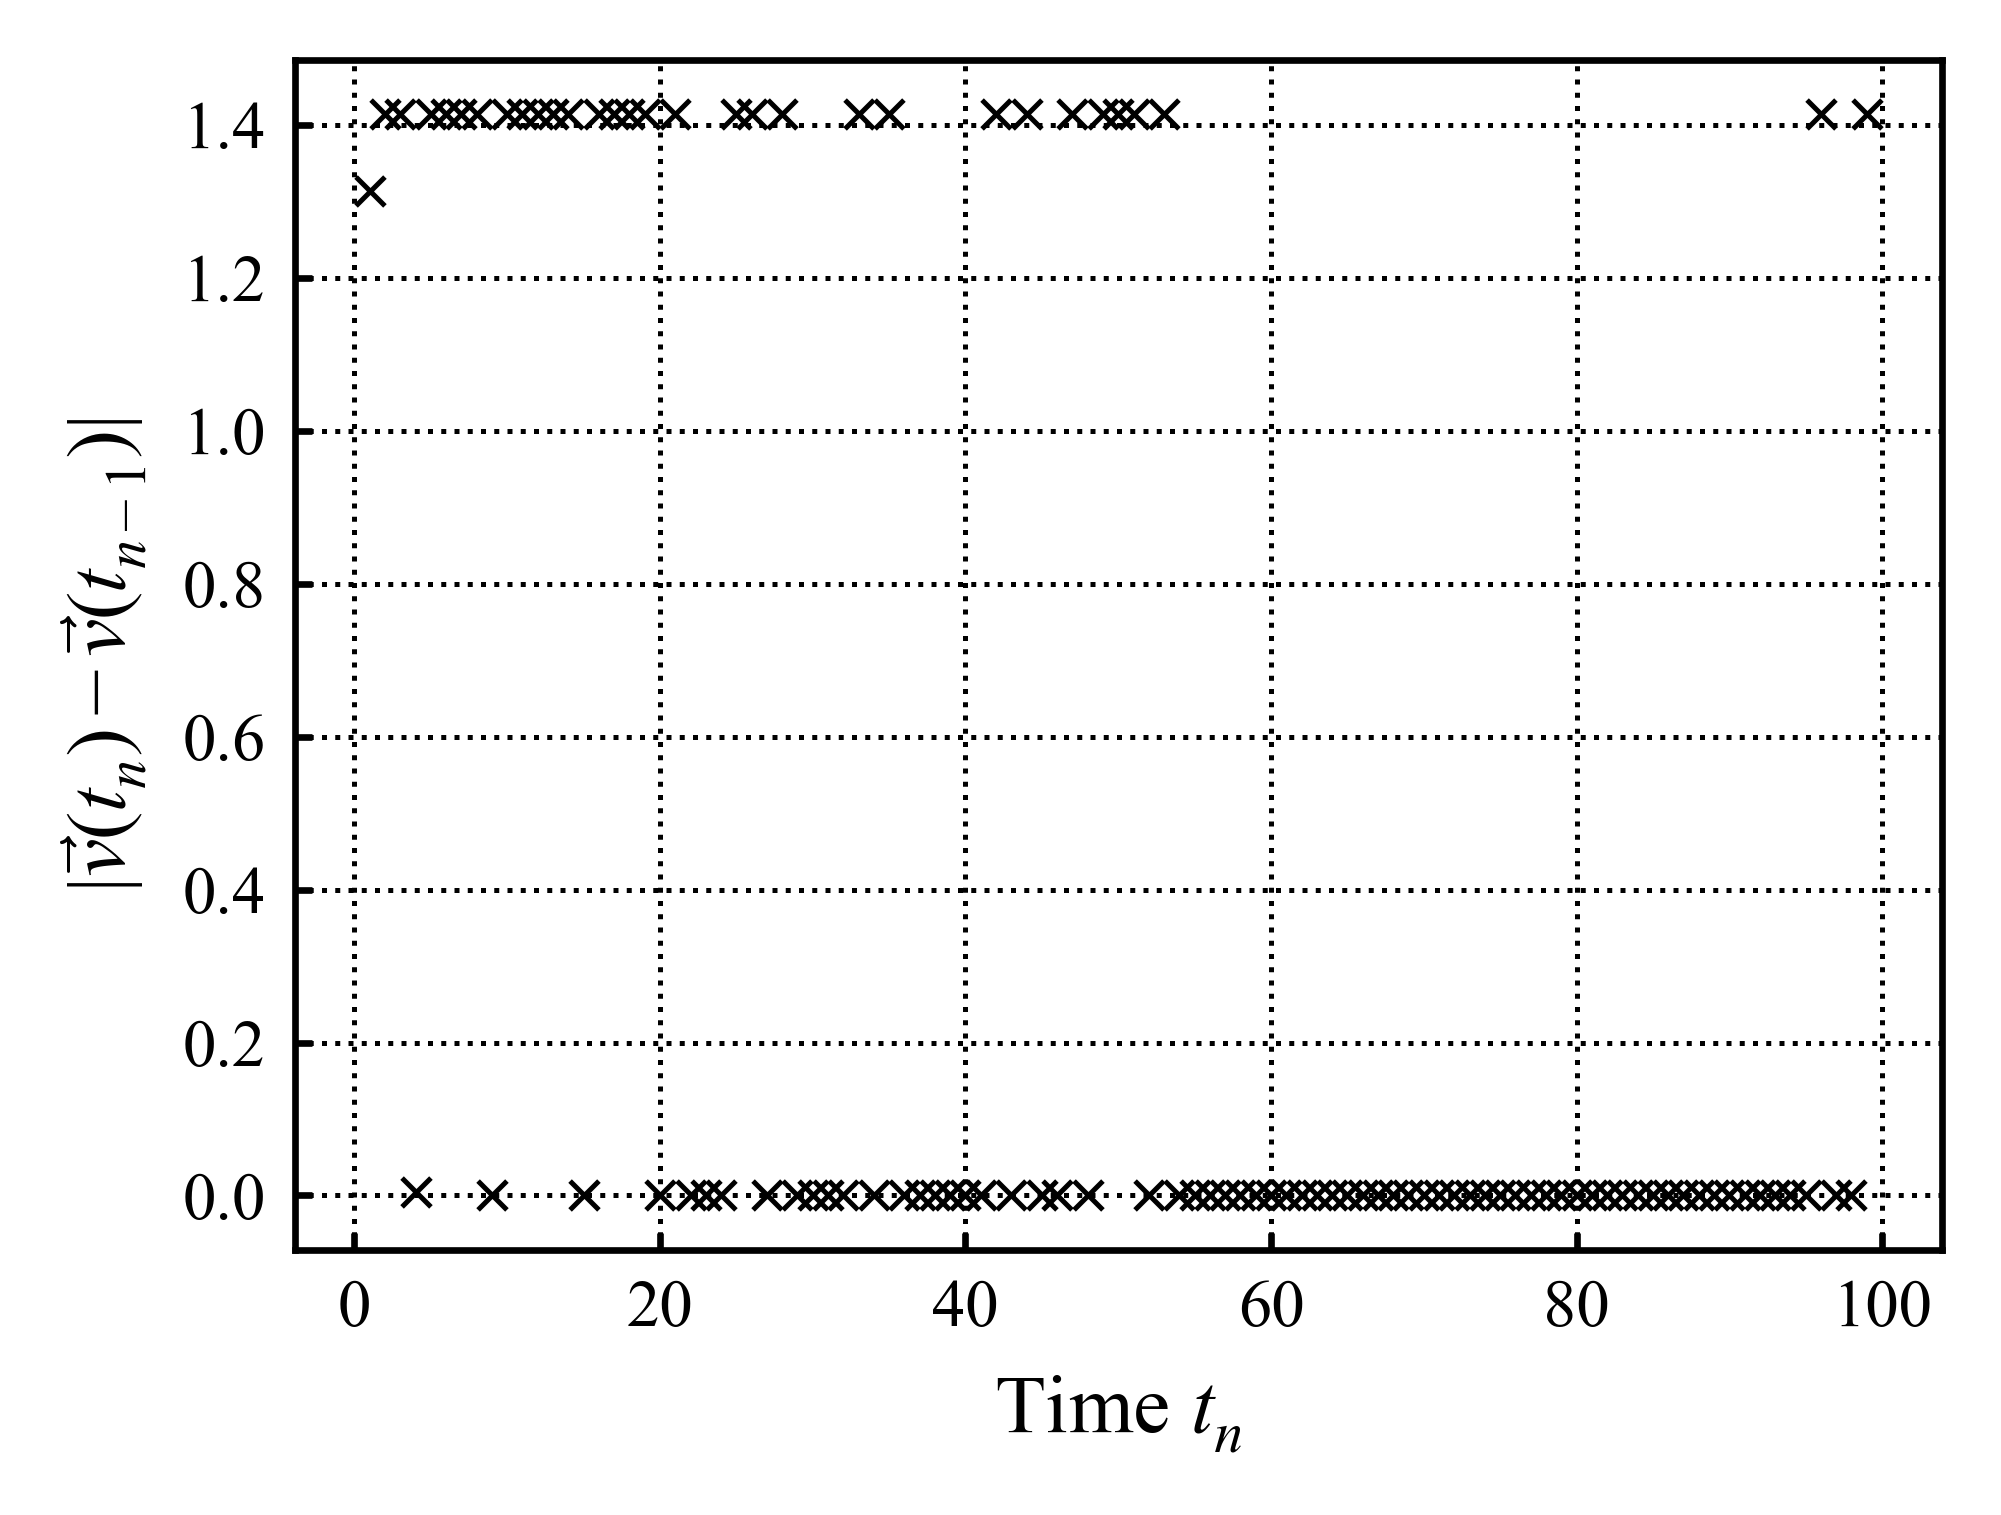
\includegraphics[keepaspectratio]{figures/eigenconvergence2Normed.png}}

}

\caption{\label{fig-eigenconvergence2Normed}Normalized second
eigenvector convergence}

\end{figure}%

Slightly different behaviour but same lack of convergence in
Figure~\ref{fig-eigenconvergence2Normed}. Last thing to try before
continuing with the first eigenvector (and validating that against other
thermalization measures) is to compare the dot product
\(\vec{v(t_{n})}\cdot\vec{v(t_{n-1})}\). Ok i may be an idiot. I am
definetely an idiot; turns out i've been using np.linalg.eig wrong; so
what I thought was the first eigenvector was simply the eigenvalues.
Reimplementing stuff with that in mind. Reexamining
Figure~\ref{fig-eigenconvergence1} and
Figure~\ref{fig-eigenconvergence2} with this in mind yields:

\begin{figure}

\centering{

\pandocbounded{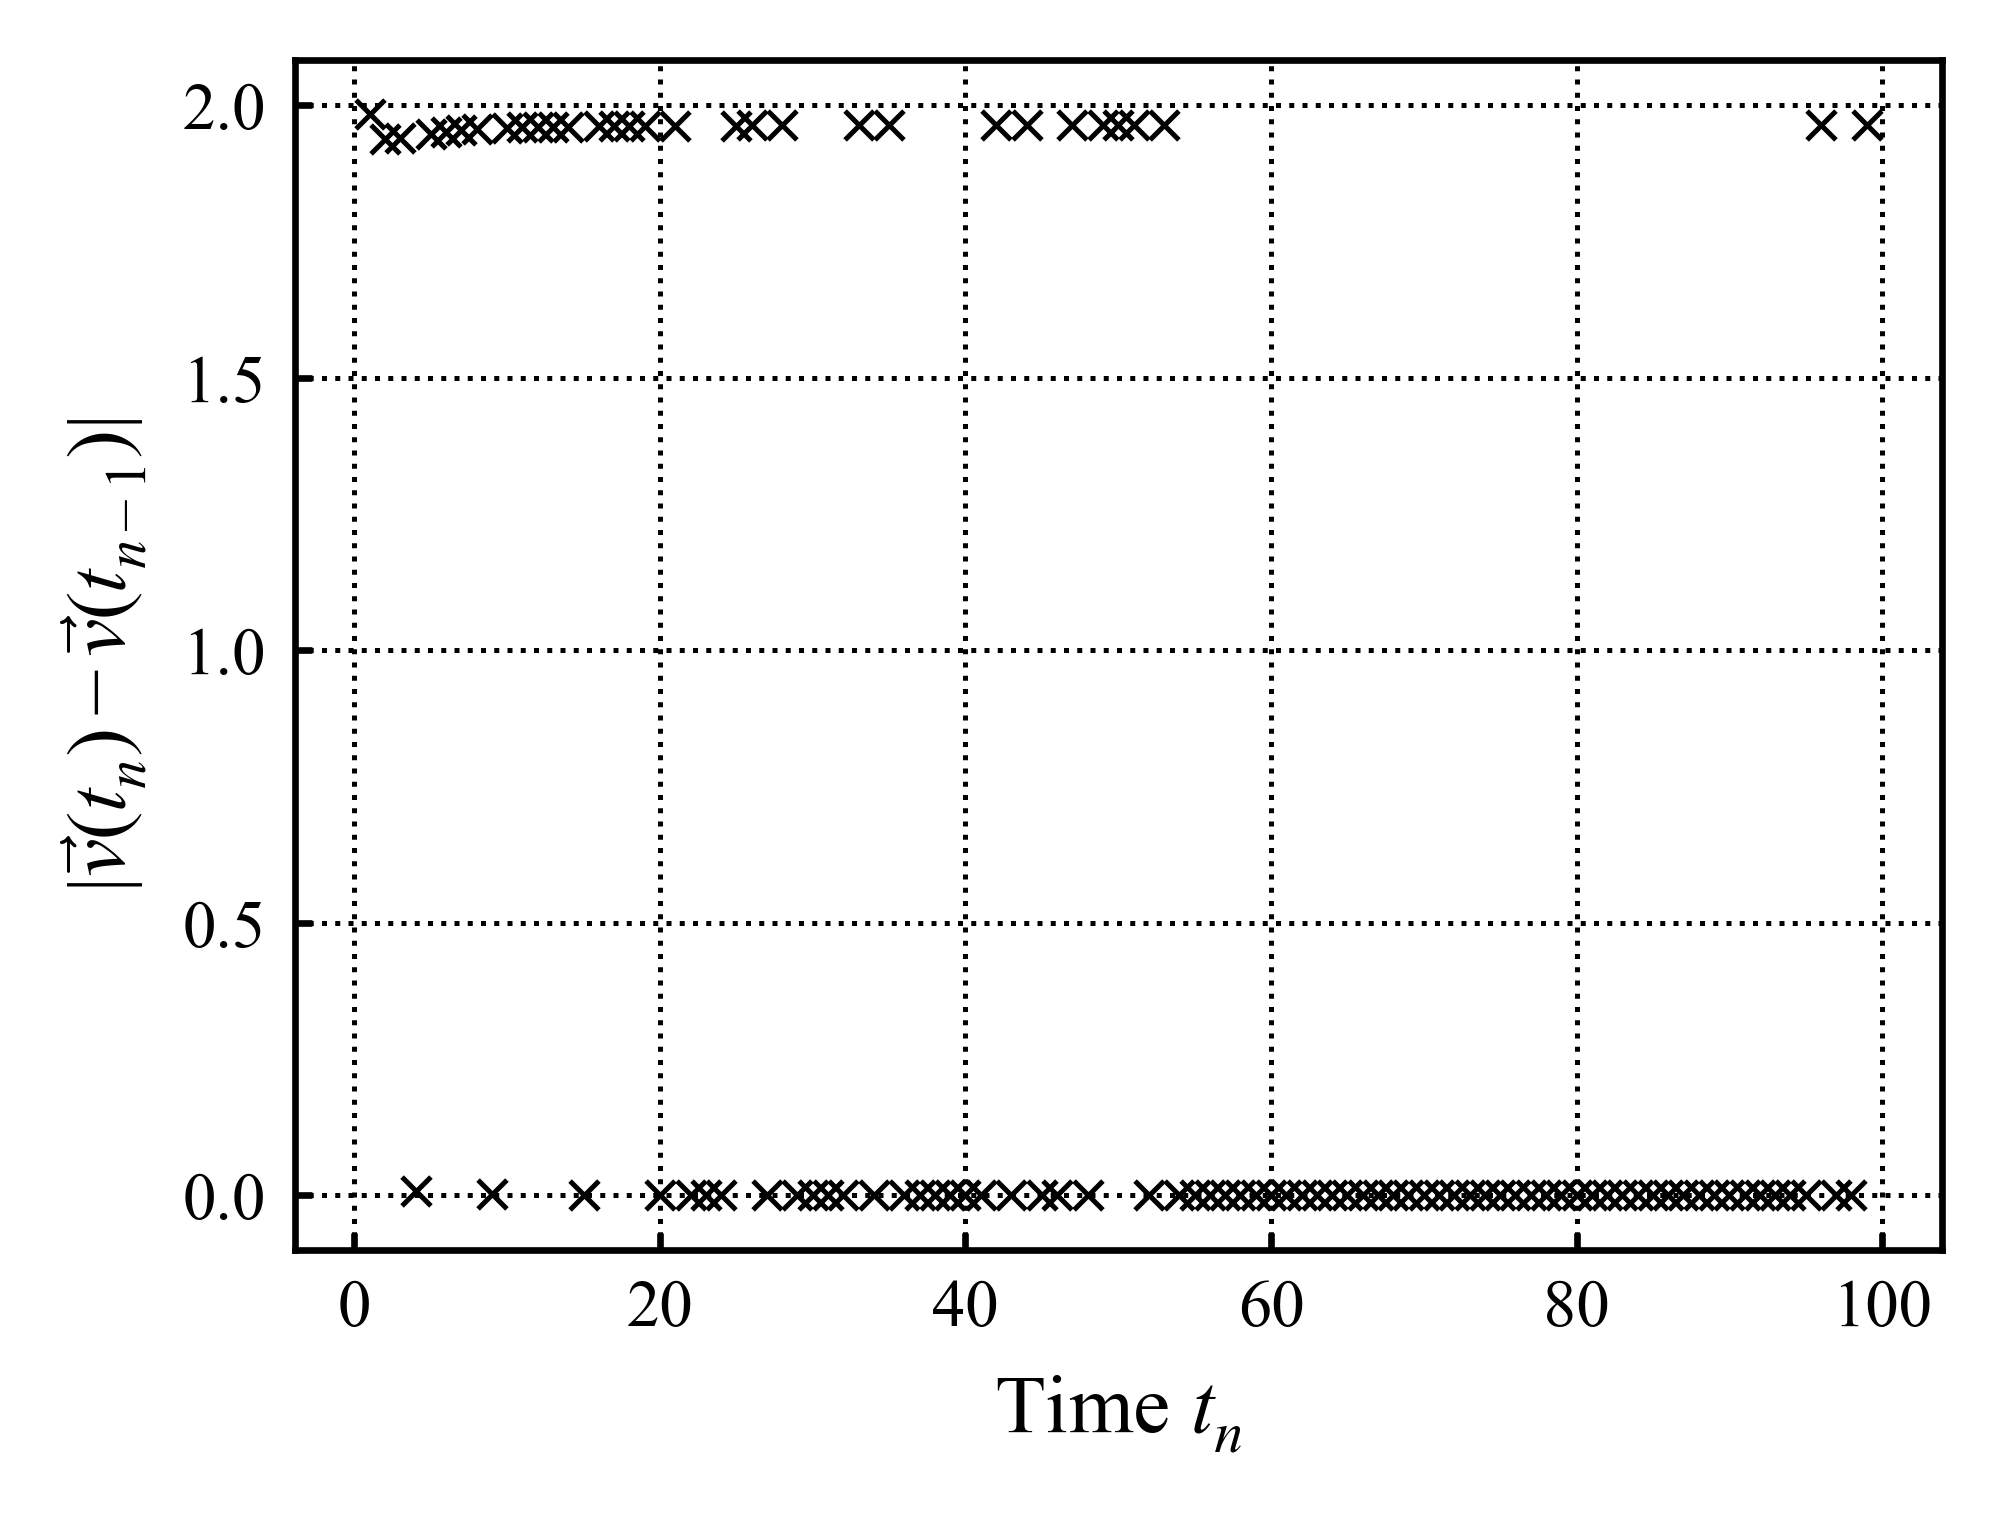
\includegraphics[keepaspectratio]{figures/eigenconvergence1Proper.png}}

}

\caption{\label{fig-eigenconvergence1Proper}First eigenvector
convergence fixed}

\end{figure}%

\begin{figure}

\centering{

\pandocbounded{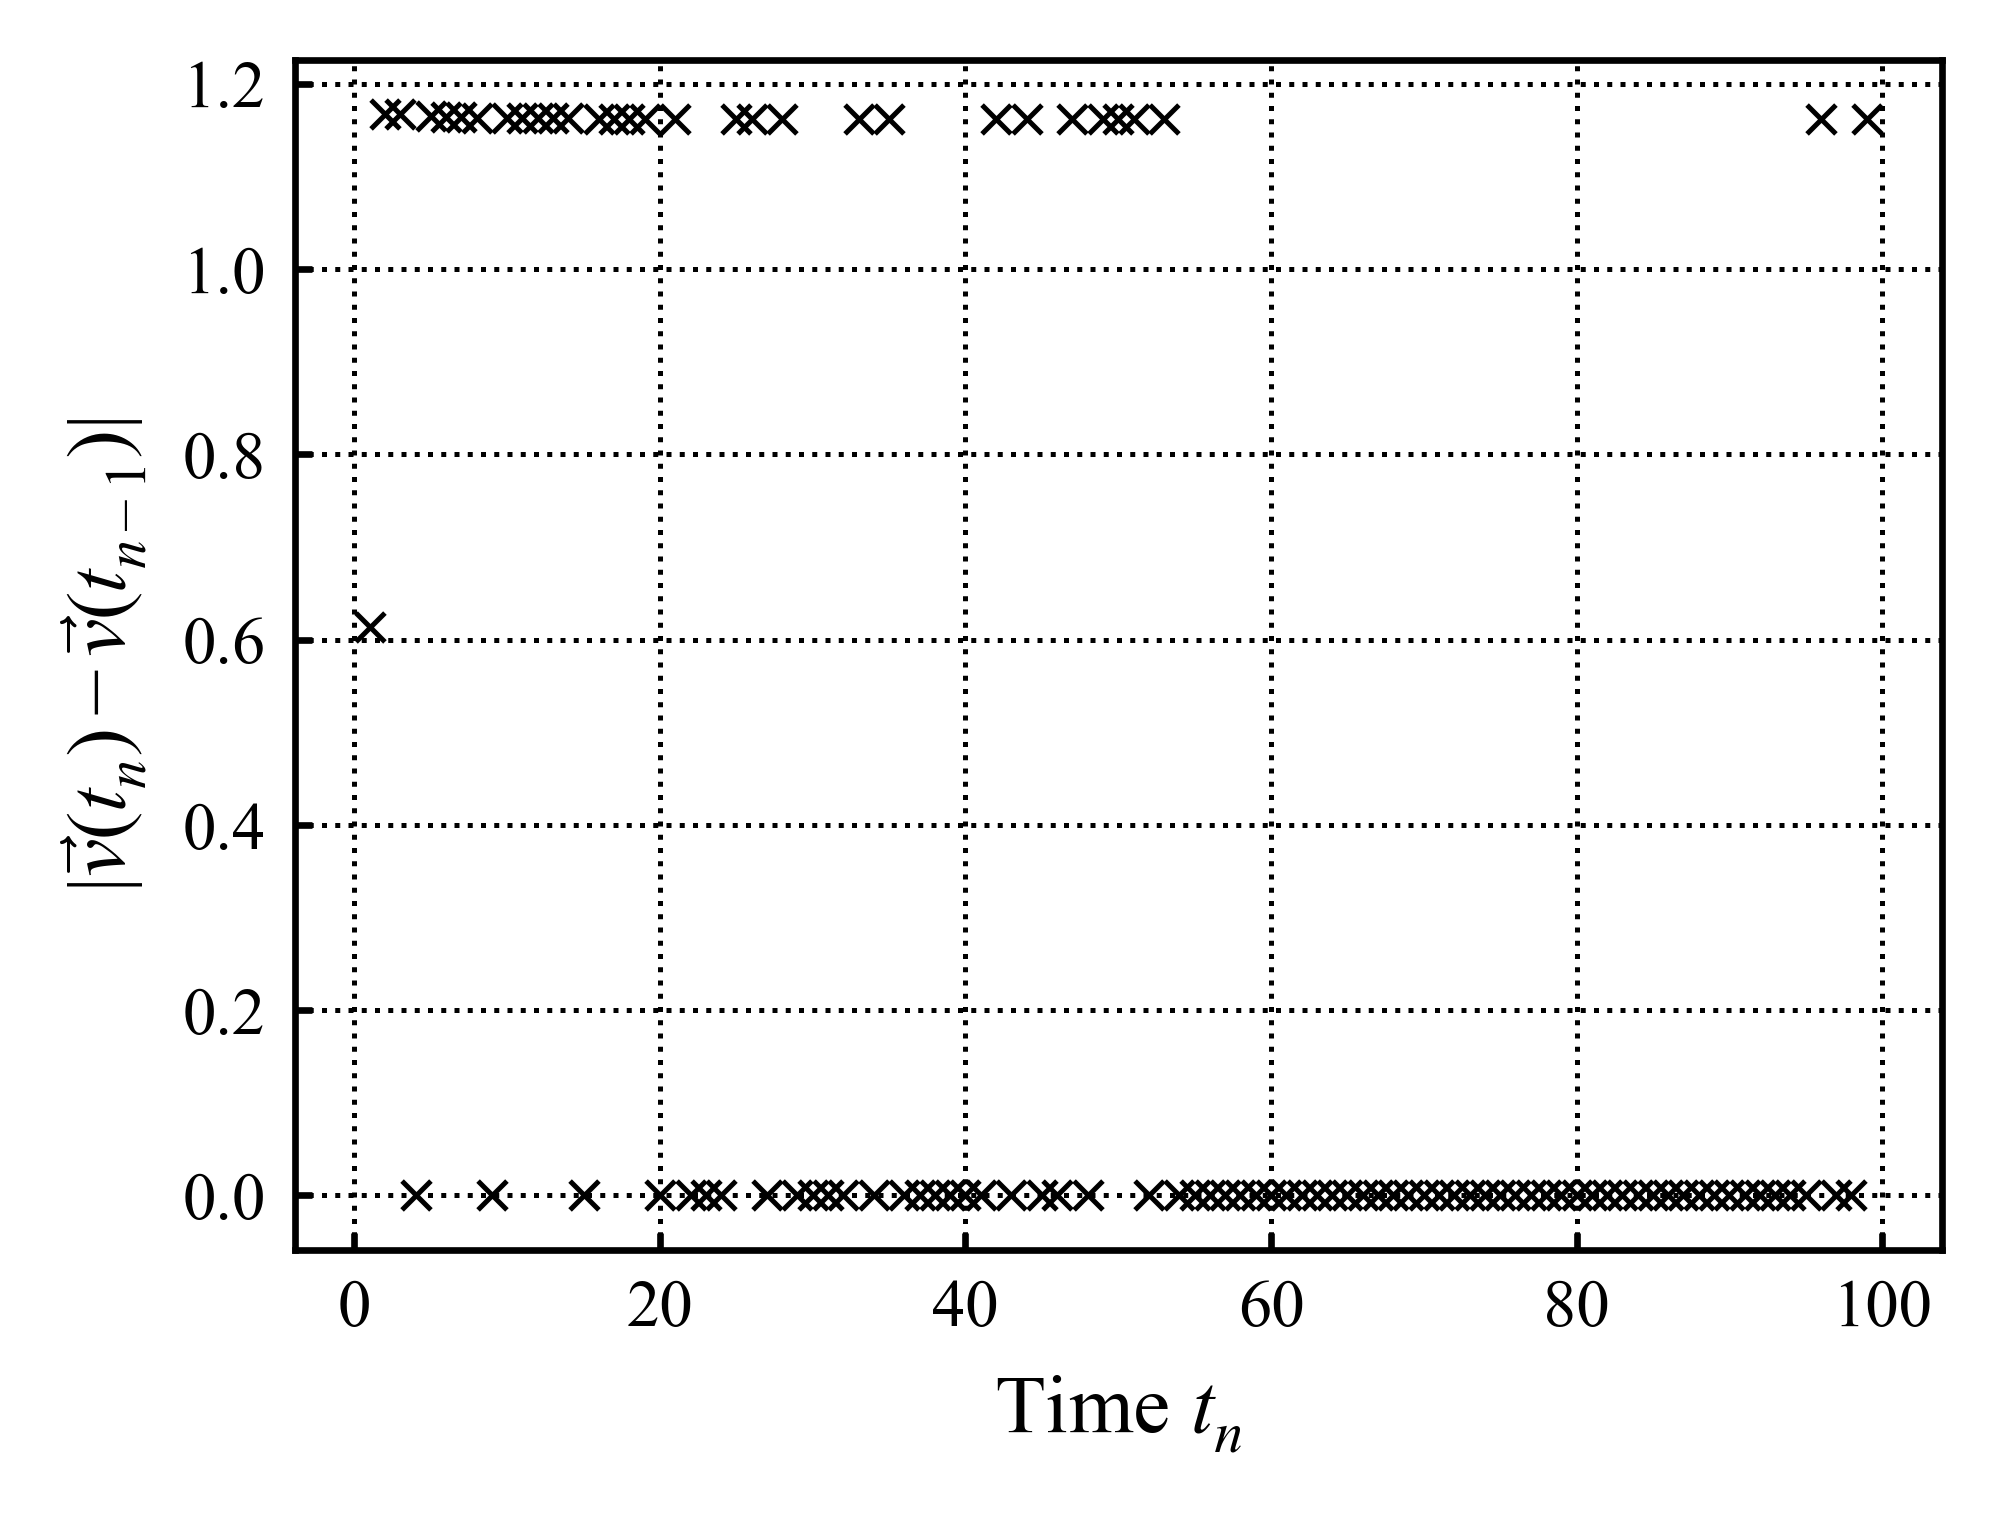
\includegraphics[keepaspectratio]{figures/eigenconvergence2Proper.png}}

}

\caption{\label{fig-eigenconvergence2Proper}Second eigenvector
convergence fixed}

\end{figure}%

Which has the same non convergence as before. I have a suspicion.

\begin{figure}

\centering{

\pandocbounded{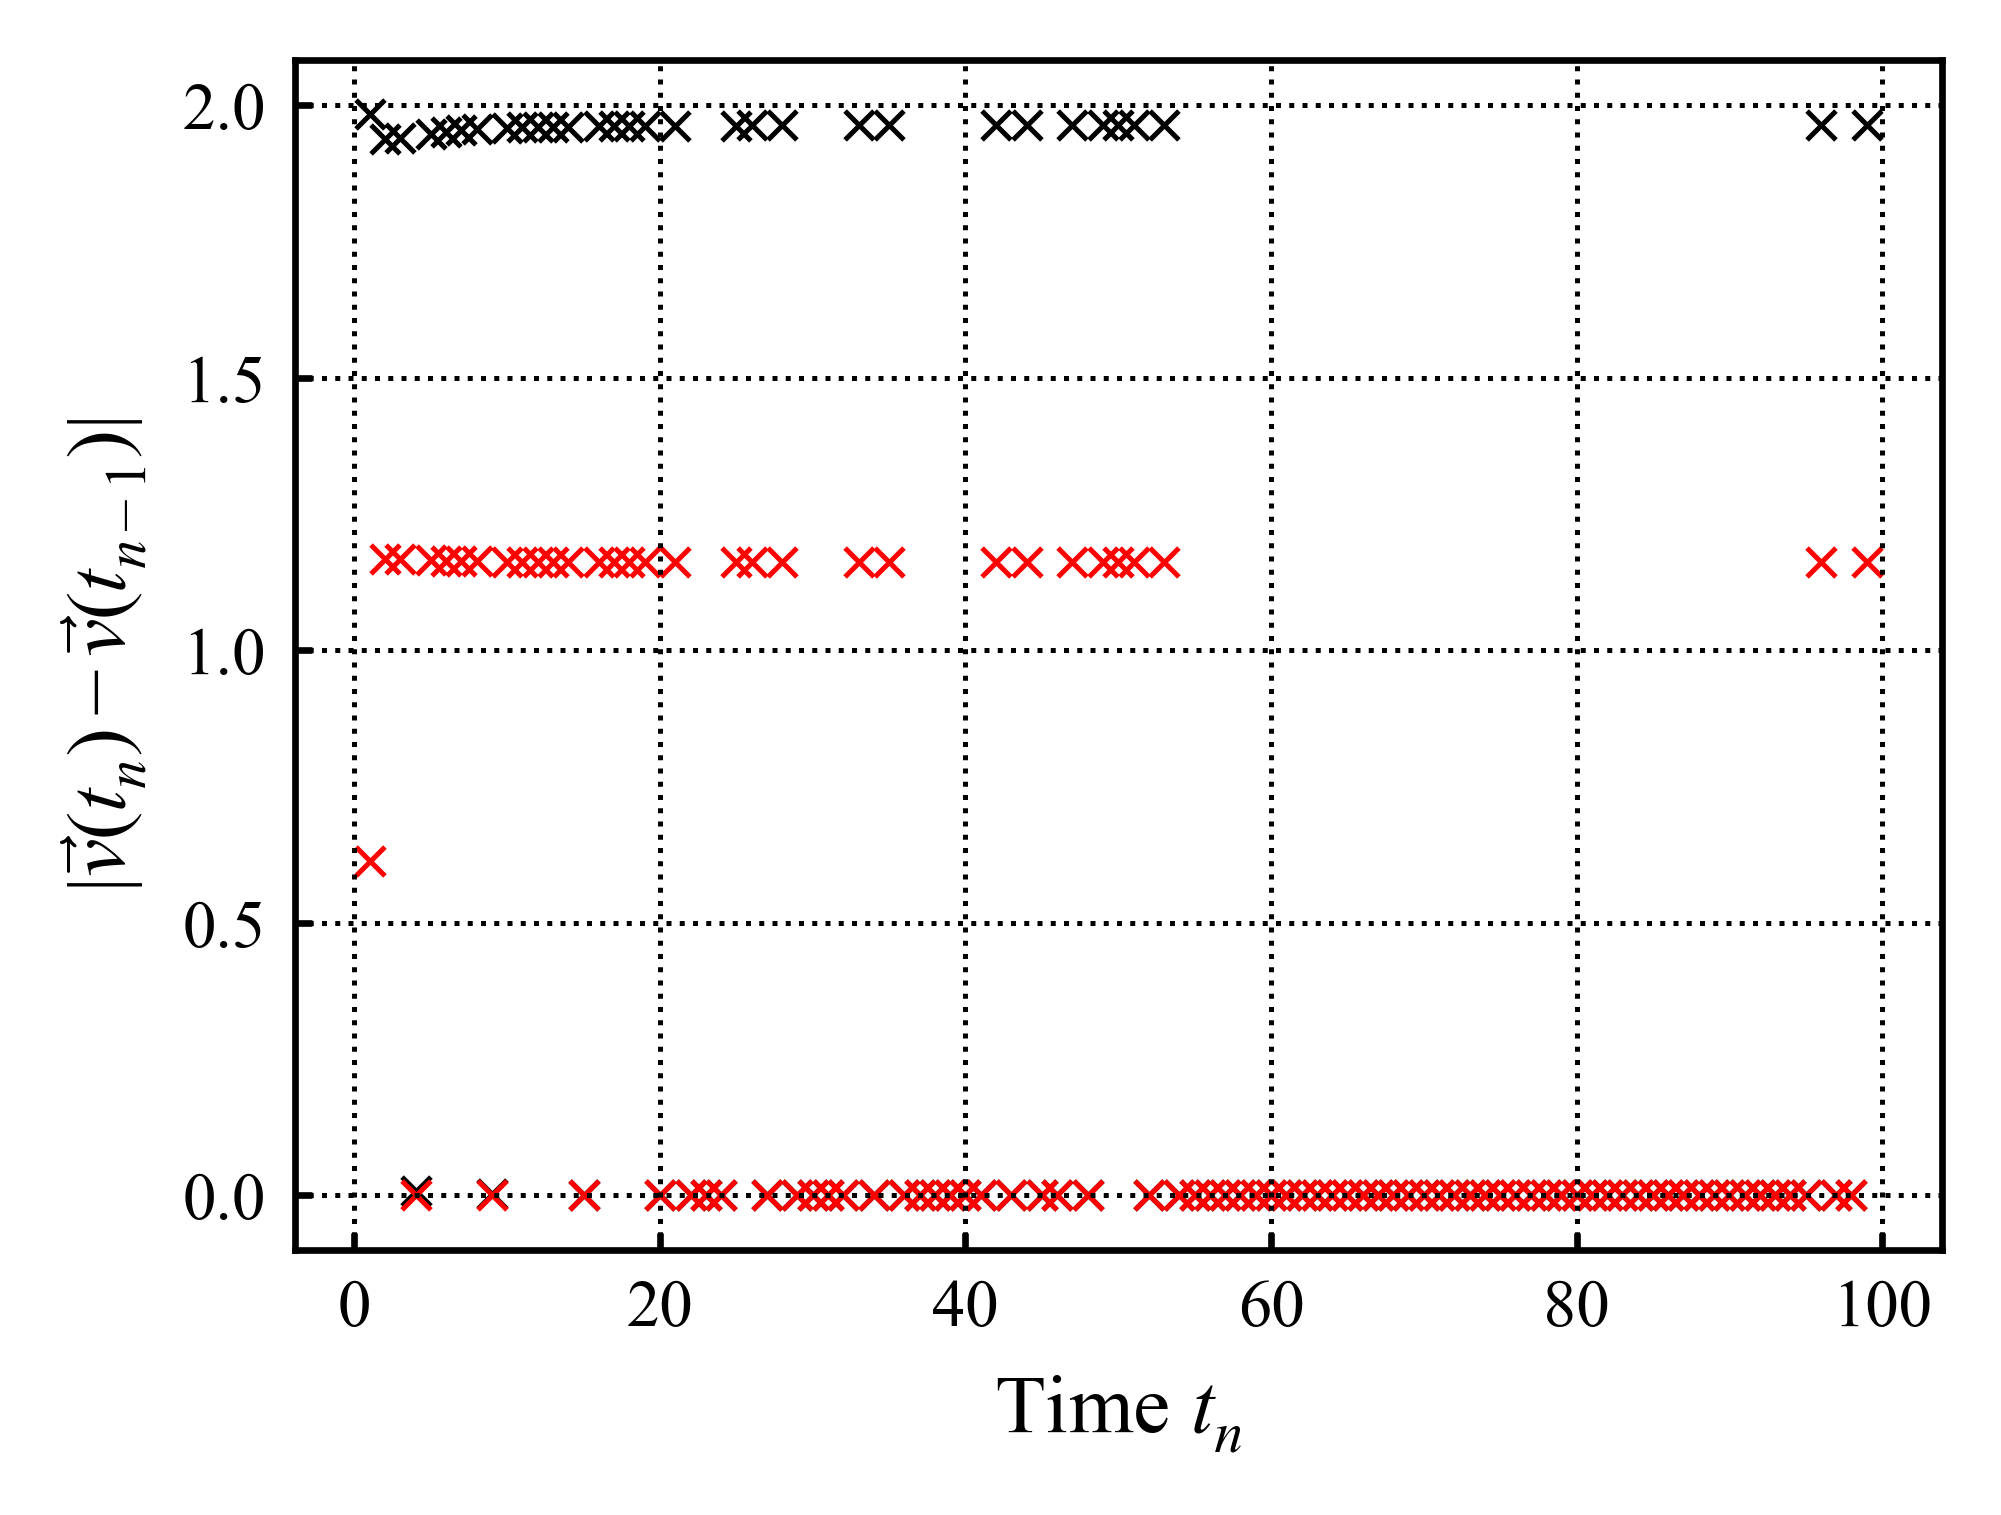
\includegraphics[keepaspectratio]{figures/eigenconvergenceBoth.png}}

}

\caption{\label{fig-eigenconvergenceBoth}eigenvector convergence, both,
black is for first eigenvector, red is for second eigenvectors}

\end{figure}%

Examining Figure~\ref{fig-eigenconvergenceBoth}, both the first and
second eigenvectors seem to stop converging for the same timesteps. I
wonder if np.linalg.eig is effectively flipping the first and second
eigenvectors at random?

I made another code mistake and wasn't pulling the correct
eigenvalues\ldots{}

The first eigenvector isn't stable, the second does converge eventually.
It is not a guarantee that the order of ``first unstable, second
stable'' will generalize; so need to algorithmically decide which is
stable, then pick the most stable value. This can be done by simply
summing up all the \(|\vec{v(t_{n})}-\vec{v(t_{n-1})}|\) values; the one
with the lowest sum is more stable so more likely to converge. Then just
need to find the time for which \(|\vec{v(t_{n})}-\vec{v(t_{n-1})}|\) is
minimised, and pick that as the ``thermalized'' eigenvector. Have
extracted this, hmmmmmmmm. This is an unphysical result. It is giving
\(\begin{bmatrix}0.13530145+2.42581405\cdot10^{-17}i \\ 0.99080448+0i \end{bmatrix}\approx\begin{bmatrix}0.13 \\ 0.99\end{bmatrix}\).
Given that state vectors are of form
\(\begin{bmatrix}1-p \\ p\end{bmatrix}\) w/\(p=\) occupation
probability, this isn't a physical result\ldots{}

I wonder if its a problem due to the relatively short test run times
used? Nope running it longer doesn't fix it. Running it w/smaller
timestep in case that is the issue. This has no effect.

I may need to rethink how i'm implementing this. Currently i'm just
finding the eigenvectors for the dynamic map for all times, seeing how
they converge, and picking the best behaved one. I am not applying
physicality constraints. A brute force approach where
\(\begin{bmatrix}1-p \\ p\end{bmatrix}\) is guessed/checked for a range
\(p\) may be better?

if so, can check dynamic map convergence instead of eigenvector
convergence; then brute force check for the physical vector closest to
the eigenvector. A binary search for a certain number of steps may be
best? Ok this just works right out of the gate.

Right, that was a side step, but that'll be a useful utility in the
future.

\subsubsection{First metrics}\label{first-metrics}

In terms of memory metrics, my instinct is to attach them to the dynamic
map ``dualSimulation'' class. The main metrics are all expressed in
terms of the dynamic map. The main exception is the ``mini metric'' of
``maximum deviation'' from the starting occupation; this ``mini metric''
depends on the specific simulated path.

That said however, I could implement it into the dualSimulation object
with an initial occupation parameter. I think i'll do it like that; its
a bit crude but should be fine. A thing worth keeping in mind is the
difference between an apparently more non-markovian dip beyond
thermalization and thermalization. As such, it's probably worth using
the presence of a relative extrema to distinguish between a
non-markovian dip and thermalization.

Ok, encountering weird effects. For context the ``standard example'' of
this maximum deviation follows in Figure~\ref{fig-maxDevFromAbove}
whereby \(n_{sys}\) starts on one side of thermalization, dips past it
before thermalizing properly.

\begin{figure}

\centering{

\pandocbounded{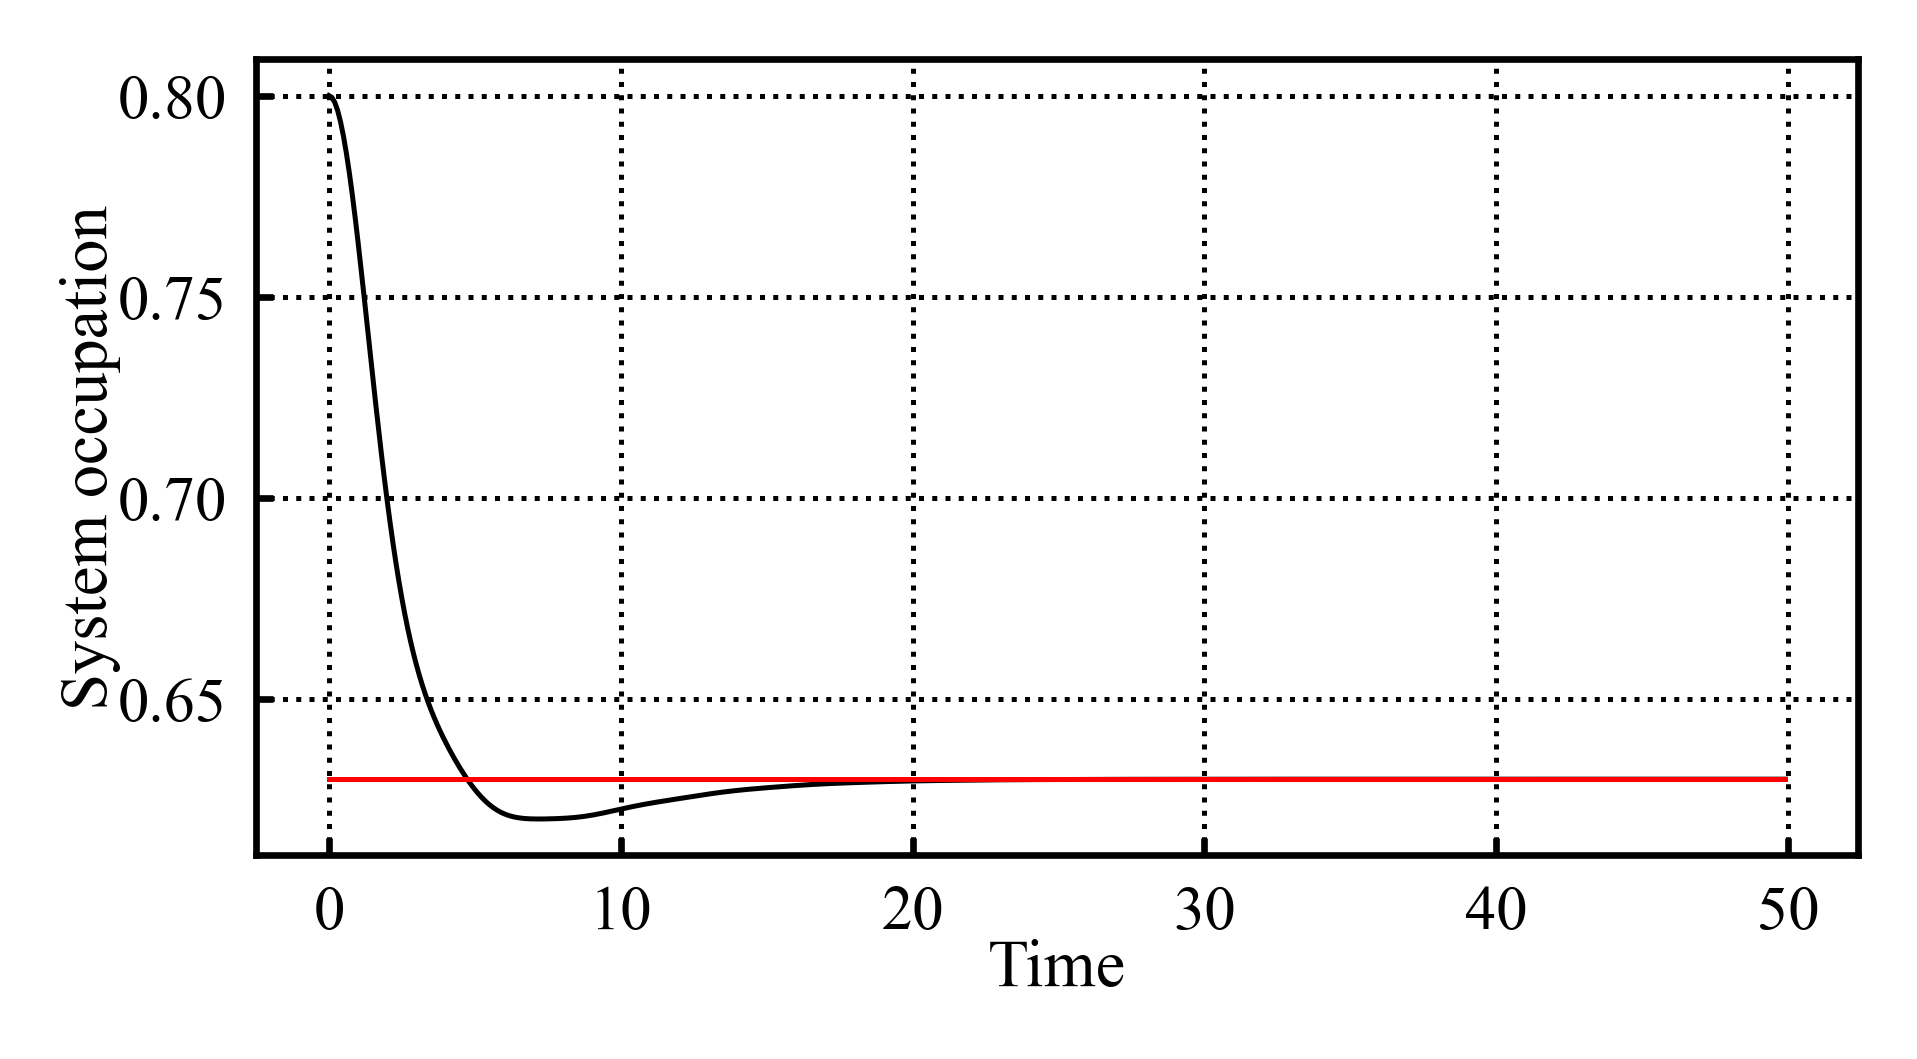
\includegraphics[keepaspectratio]{figures/maxDevFromAbove.png}}

}

\caption{\label{fig-maxDevFromAbove}Evolution from
\(n_{sys}(0)>n_{therm}\) for
\(f_{pre}=0.2, \beta=10, \mu=0.1, D=2, \epsilon=0\)}

\end{figure}%

In this context, the ``maximum deviation'' is the gap between initial
occupation and that particular hump. However trying to reproduce this
effect from below yielded:

\begin{figure}

\centering{

\pandocbounded{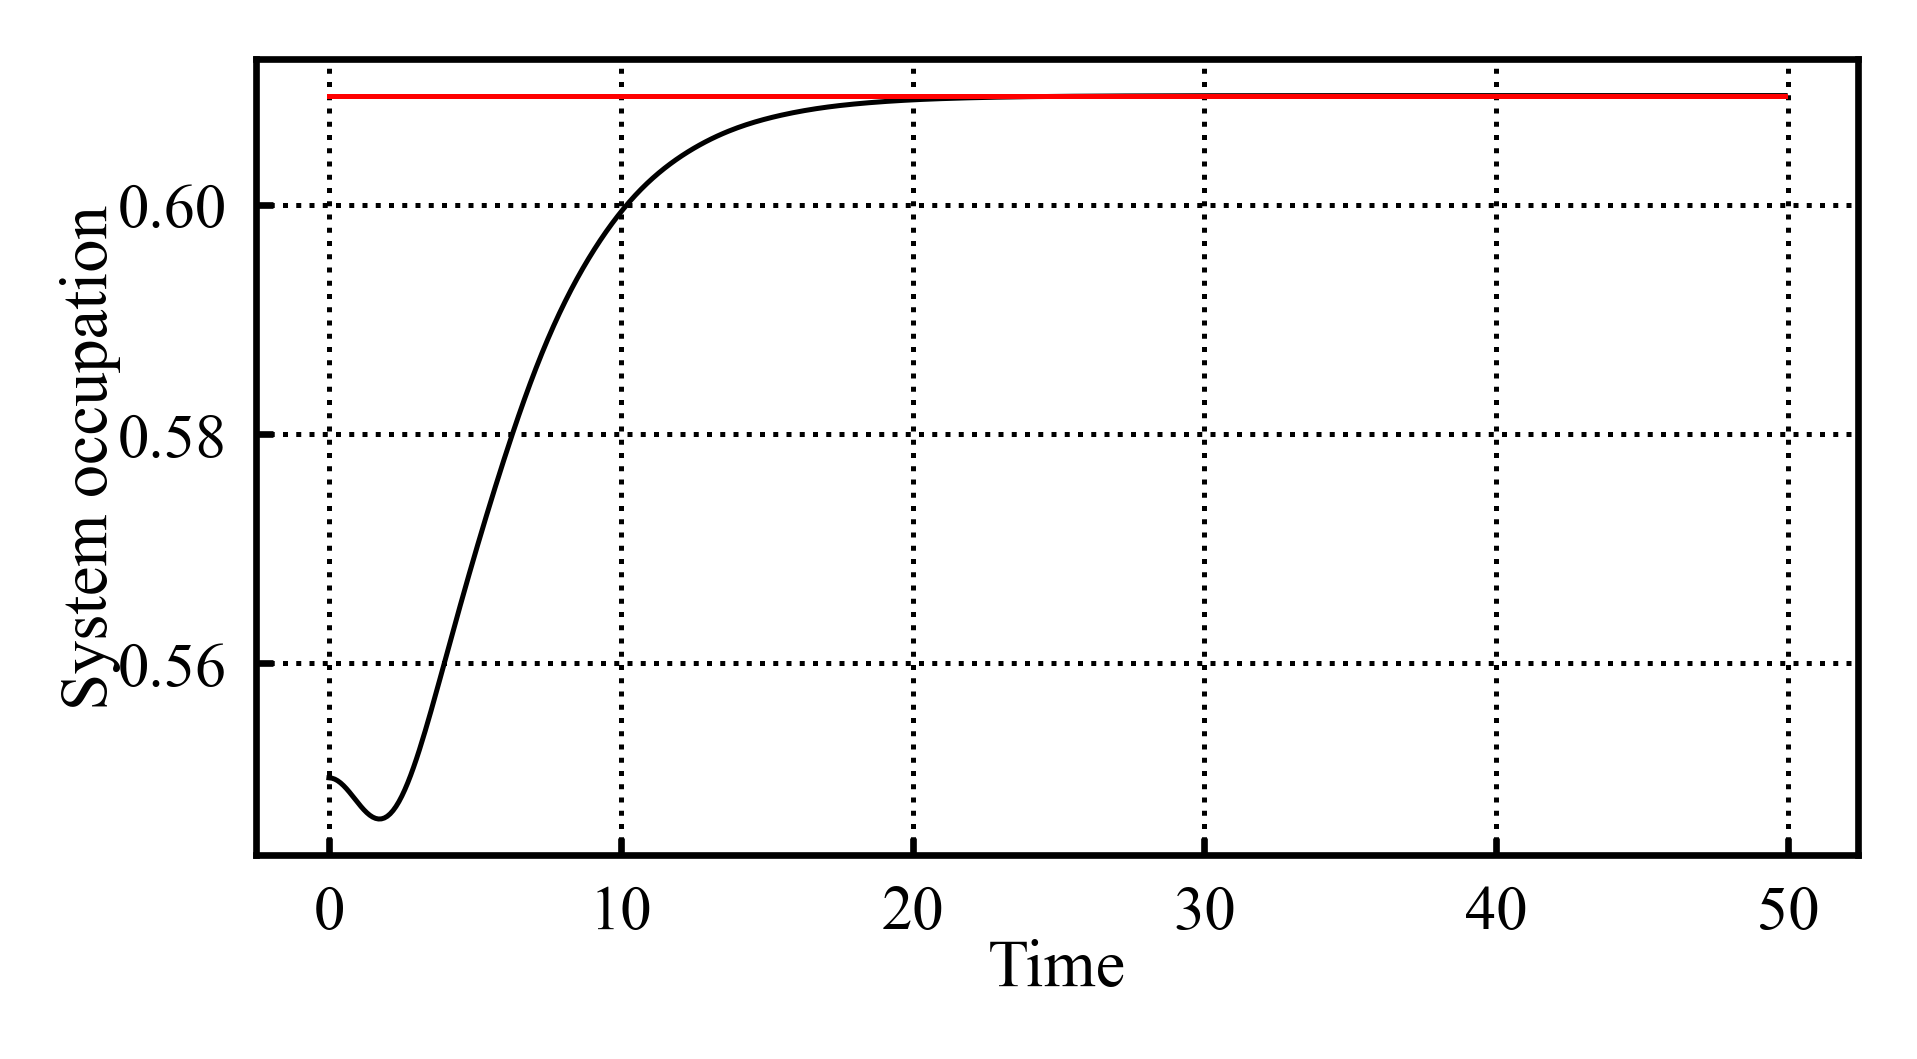
\includegraphics[keepaspectratio]{figures/maxDevFromBelow.png}}

}

\caption{\label{fig-maxDevFromBelow}Evolution from
\(n_{sys}(0)<n_{therm}\) for
\(f_{pre}=0.2, \beta=7, \mu=0.1, D=2, \epsilon=0\)}

\end{figure}%

Which moves away from thermalization first before thermalizing normally.
My naive instinct was that it should be possible to symetrically flip
Figure~\ref{fig-maxDevFromAbove}, however that doesn't seem to be the
case\ldots{} This brings some degree of ambiguity in terms of what this
``max deviation mini metric'' is meant to be measuring. Going to take
some time to examine these effects for various initial occupations,
because i wonder if these ``bumps'' are being drawn to similar values
regardless of where the occupation starts.

\begin{figure}

\centering{

\pandocbounded{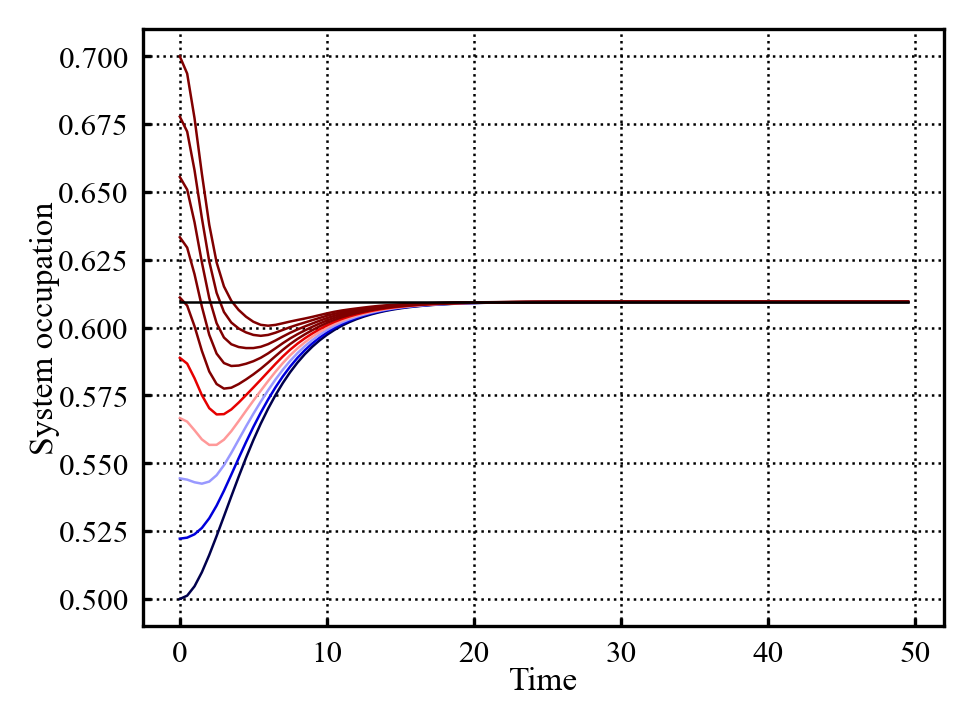
\includegraphics[keepaspectratio]{figures/humpDualSimulation_rangeInitial.png}}

}

\caption{\label{fig-humpDualSimulation_rangeInitial}Evolution from range
of \(n_{sys}(0)\) for
\(f_{pre}=0.2, \beta=7, \mu=0.1, D=2, \epsilon=0\)}

\end{figure}%

Plotting for a range of initial occupations yields
Figure~\ref{fig-humpDualSimulation_rangeInitial} which does lend the
idea that the ``bumps'' are being drawn to some curve credence\ldots{}

I'm unsure why this is, however it does expand the initial idea of bumps
past thermalization being what needs measuring. In some way this max
deviation represents some deviation from a ``bumpless'' evolution.
Unfortunately it doesn't seem simple to substract ``w/out bumps'' data
from ``w/ bumps'' data in order to try to isolate the ``bump'' signal.
For instance changing the prefactor will necessarily change the
timescale of the dynamics requiring rescaling if i'd want to compare
them directly.

All that said, i think for this ``mini metric'' simply doing the
deviation from a relative extrema regardless of the shape should be
fine?

Have quickly implented a default ``examine maximum deviation from
initially thermalized state'' utility and plotted it as:

\begin{figure}

\centering{

\pandocbounded{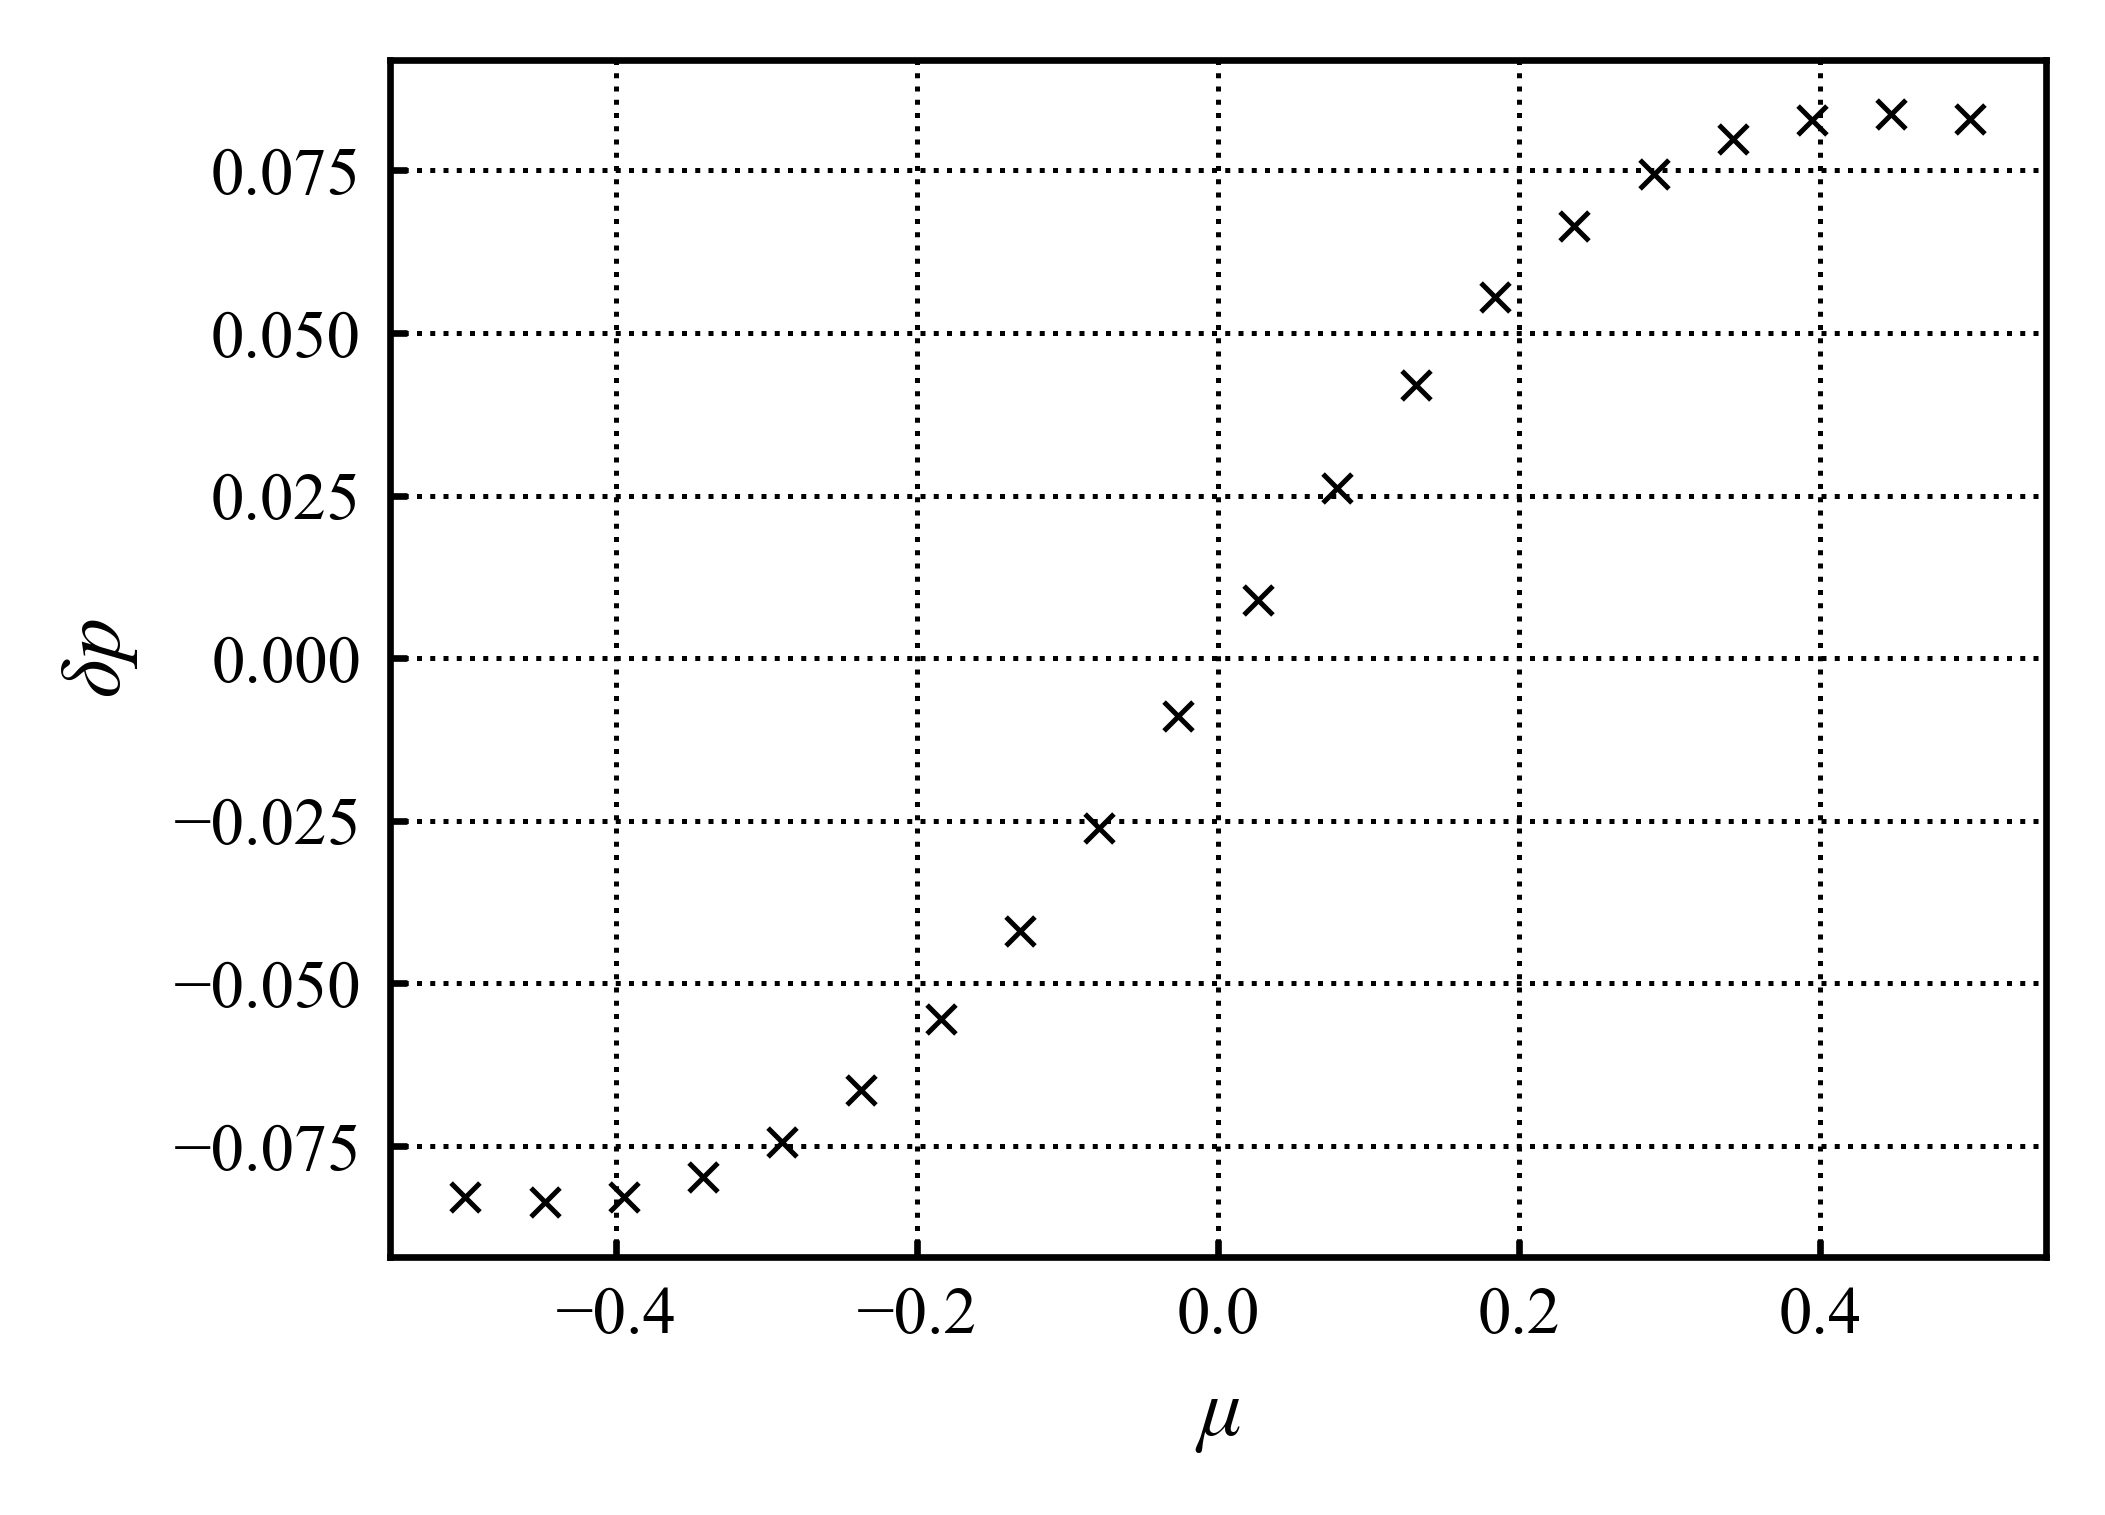
\includegraphics[keepaspectratio]{figures/maxDevOverMu.png}}

}

\caption{\label{fig-maxDevOverMu}Max deviation from
\(n_{sys}(0)=n_{therm}\) for different \(\mu\) for
\(\beta=7, f_{pre}=0.2, D=2\)}

\end{figure}%

Interesting how well behaved it is. I wonder if i decrease the
temperature if it will show a sharper curve?

\begin{figure}

\centering{

\pandocbounded{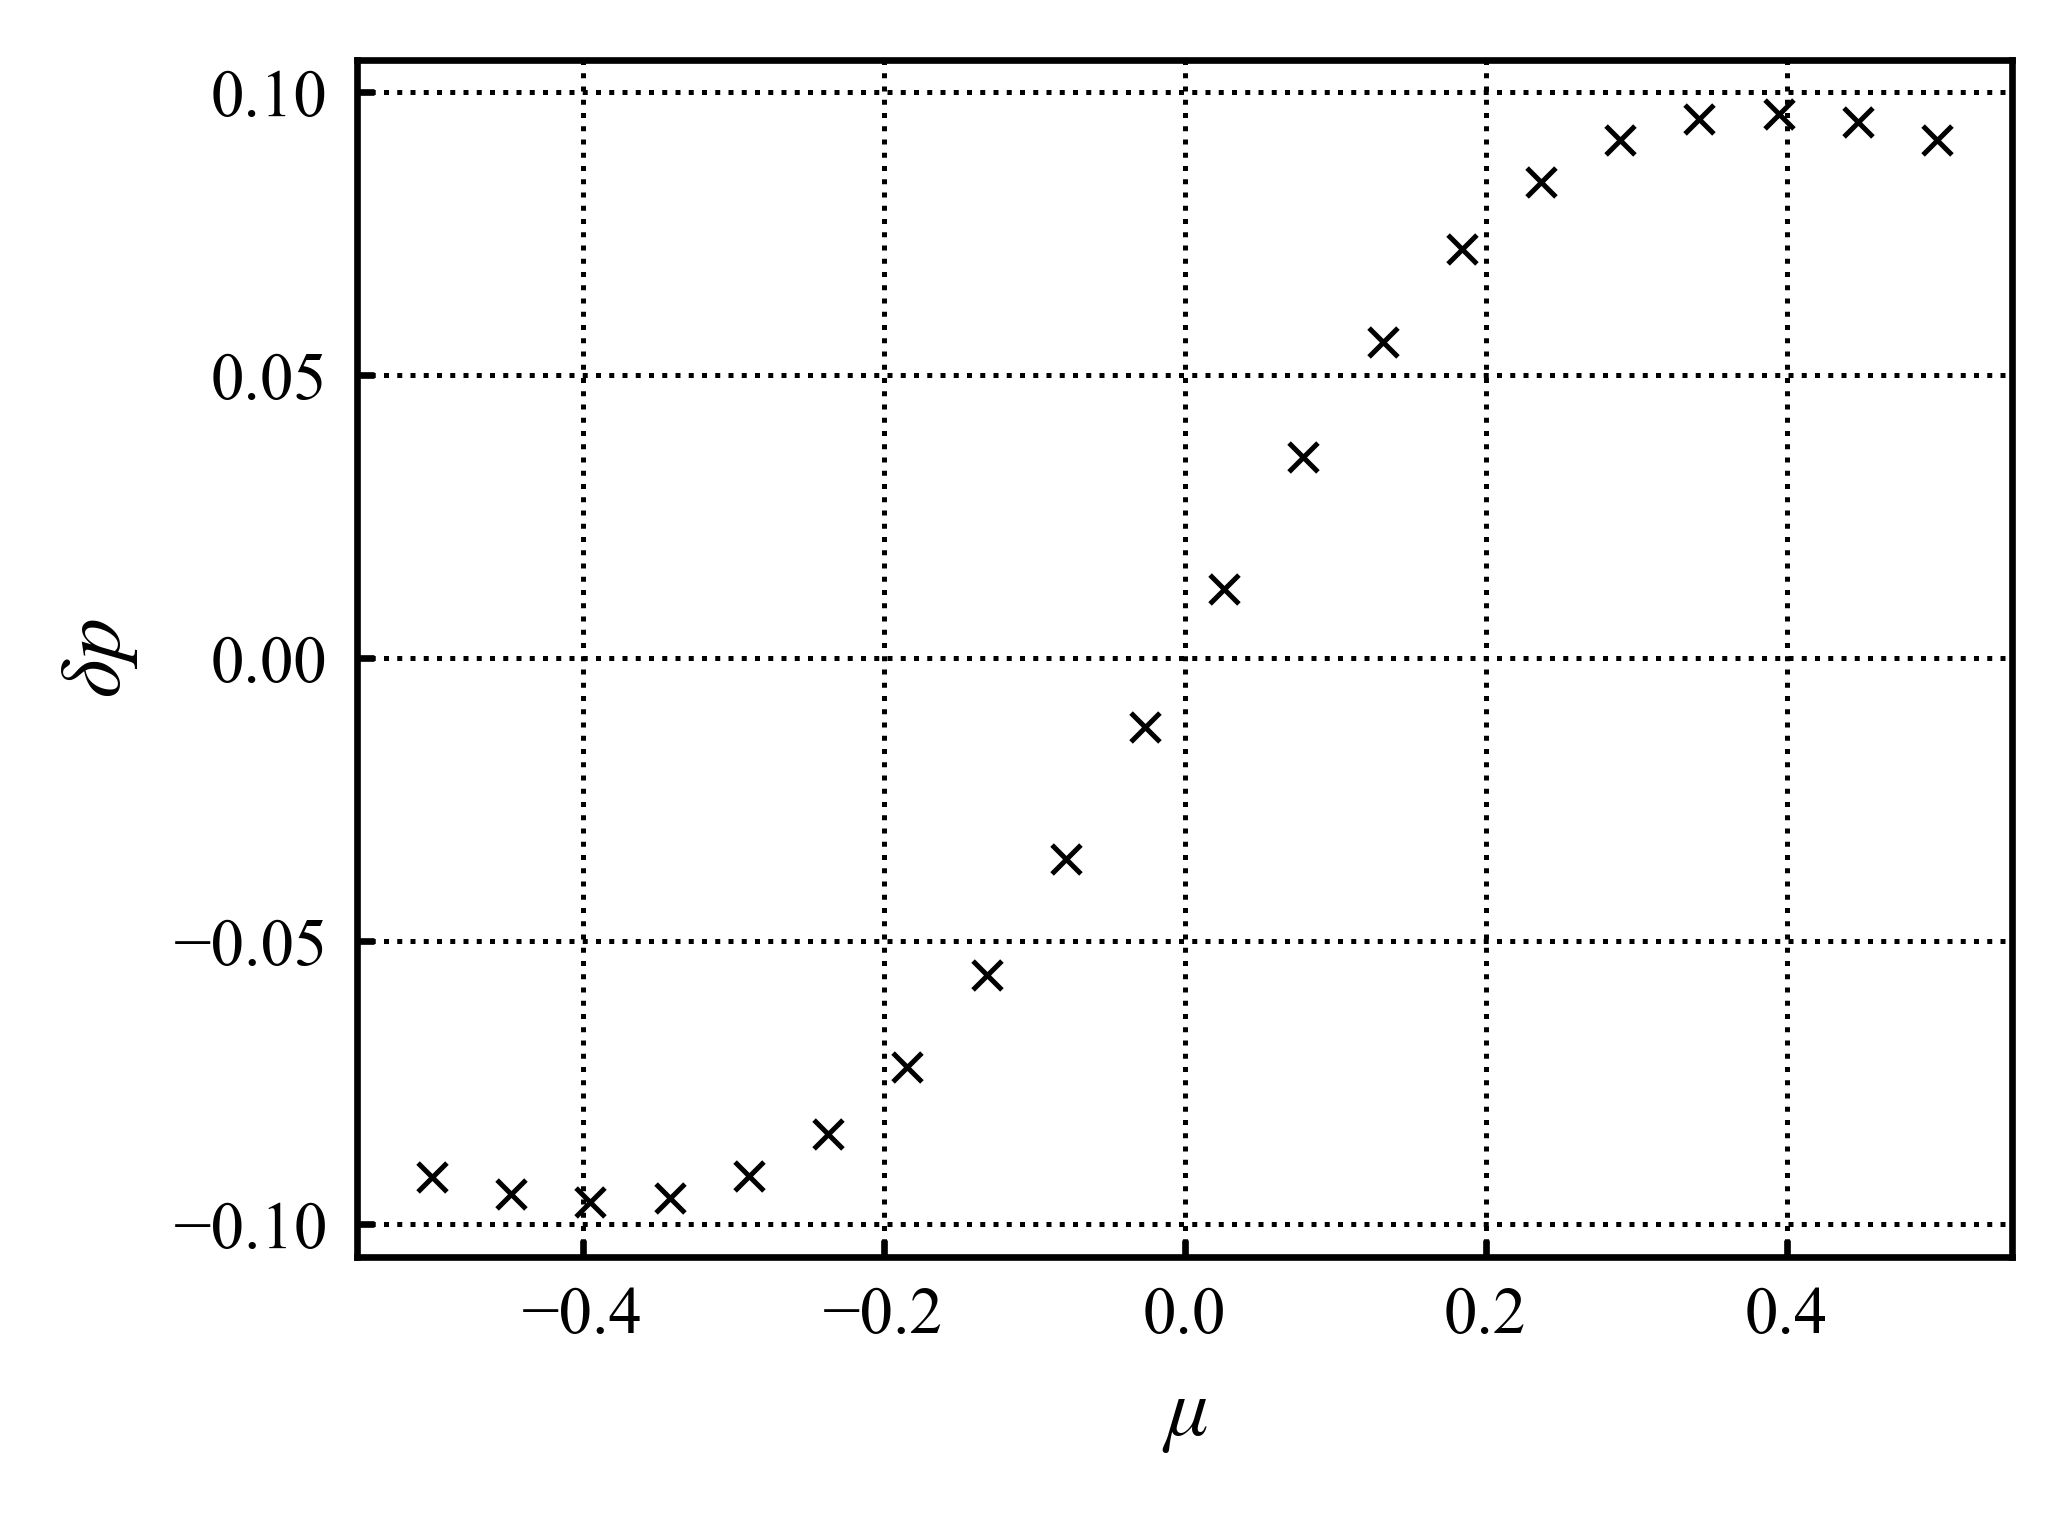
\includegraphics[keepaspectratio]{figures/maxDevOverMuBeta10.png}}

}

\caption{\label{fig-maxDevOverMuBeta1-}Max deviation from
\(n_{sys}(0)=n_{therm}\) for different \(\mu\) for
\(\beta=10, f_{pre}=0.2, D=2\)}

\end{figure}%

Well thats interesting\ldots{} its not a logistic function; but I doubt
its periodic\ldots{} Actually, examining (Strachan, Purkayastha, and
Clark 2025) fig 2 this is consistent. It seems to be generally of the
right order of magnitude and behaviour at first inspection. And that is
enough for today, will get back to this another time.

\subsection{08/11/2026}\label{section-3}

Think i'm going to do some minor code restructuring/cleanup today. Main
thing is that i want the ``code utilities'' that standardise simulation
and data calls to be a bit cleaner. Particularly i currently do not make
use of the save/load utilities. Given that compute times are increasing,
being able to load in standard simulation sets for analysis will likely
be useful.

an additional related bit of work is restructuring how i'm organising my
saved data. Currently its all in a disorganised folder. I think most of
whats currently there can be moved to a ``pathfinding'' data folder, and
a better organisational structure can then be implemented for the long
term.

Have implemented and tested some loading utilities. Currently the
utilities also have some functions which can easily generate and
simulate parameter variations for a single parameter. This is fine
currently, but I do want the option of varying multiple parameters over
a \(d>1\) parameter space. As such I want to rethink exactly how i'm
storing these ``datasets'' for multiple runs.

Currently with 1D variations (1 parameter is varied) a list of parameter
args and a list of simulations or dualSim objects is sufficient. However
if I end up making multidimensional parameter spaces, that approach may
get cumbersome.

It may be worth implementing a ``dataset'' class which handles this.
This would keep track of the coordinates in parameter space and their
corresponding simulation/dual simulation. Given that i'll mostly be
working with the dynamic map from now on, I think it's mainly worth
implementing it for the dualSim object. If i need this functionality for
the simulation class, i can implement that later.

This ``dataset object'' should ideally:

\begin{itemize}
\tightlist
\item
  store points in parameter space - this includes both the parameters
  and the attached dualSimulation object

  \begin{itemize}
  \tightlist
  \item
    this will also require constructing/running this space in the first
    place, i think this construction should follow a ``grid''
    construction - i give it lists of parameter variations (I.E,
    spectralPrefactor: {[}0.01, 0.02\ldots{]}, beta: {[}0, 0.1\ldots{]})
    then it will construct all combinations of points (I.E {[}{[}(0.01,
    0), (0.01, 0.1){]} \ldots{} {[}(0.02, 0), (0.02, 0.1){]} \ldots{]})
  \end{itemize}
\item
  be able to save itself to folder/file
\item
  be able to load itself from folder/file
\item
  handle queries to the data:

  \begin{itemize}
  \tightlist
  \item
    should be able to request dualSim associated w/specific coordinates
    in parameter space
  \item
    should be able to request ``slices'' of the data - specify some
    fixed parameter and let the rest vary
  \end{itemize}
\end{itemize}

This will take a bit of time to implement robustly, however it should
make the rest of this project a lot easier. The main question then is
how do i want to structure the internal ``parameter space''
datastructure. It will need to be spat out to a 1D list asp for
saving/loading purposes. However it'd be nice to be able to access the
data in the full dimensional space. Pandas may help, pandas dataframe
w/each row a different point; columns for all the parameters, one column
for the corresponding dualSim object. this would let me access data
using pandas filtering functionality.

Have started implementing this, however not finishing today i think.

\phantomsection\label{refs}
\begin{CSLReferences}{1}{0}
\bibitem[\citeproctext]{ref-DavidMpemba2026}
Strachan, David J., Archak Purkayastha, and Stephen R. Clark. 2025.
{``Non-{Markovian} {Quantum} {Mpemba} {Effect}.''} \emph{Physical Review
Letters} 134 (22): 220403.
\url{https://doi.org/10.1103/PhysRevLett.134.220403}.

\end{CSLReferences}




\end{document}
